%
% Modellbildung
%
% @version 1.0
% @author dmayer
% @created 29. Dezember 2015

\setchapterpreamble[o]{%
\dictum[--- \textsc{Norbert Wiener}, \emph{US-amerikanischer Mathematiker}]{\Gun Das beste Modell für eine Katze ist eine Katze; möglichst dieselbe Katze. \Gob}}
\renewcommand{\chapterheadstartvskip}{\vspace*{2cm}}

\chapter{Modellbildung und Simulation}
\label{chap:modellbildung}

Ziel dieses Kapitels ist es, ein hinreichend exaktes Modell zur Berechnung der Raumtemperatur in  Raum K004b zu bilden. Die Modellbildung soll physikalisch motiviert sein und daher auf den thermodynamischen Prozessen des Raumes mit der Außenumgebung und der Anlage aus Kapitel \ref{chap:anlagendesign} basieren. Es soll außerdem speziellen Anforderungen genügen, die eine Modellprädiktive Regelung der Anlage ermöglichen.

Zunächst wird ein einfaches Grundmodell für einen hypothetischen Raum gebildet, dass anschließend schrittweise erweitert und an den bestehenden Raum angepasst wird. Nachdem eine Anpassung an die realen Einflussgrößen erfolgt ist, wird die Güte des Models mithilfe einer Simulation abgeschätzt und schließlich durch eine Parameterschätzung verbessert. Zum Abschluss wird überprüft, ob sich das Modell für den Einsatz einer Modellprädiktiven Regelung mit \textsc{JModelica.org} eignet.


\section{Modellbildung}

\subsection{Anforderungen an das Raummodell}

Das Modell hat die triviale Aufgabe die realen Vorgänge und den Temperaturverlauf hinreichend genaue zu beschreiben. Hinreichend bedeutet, dass das Modell eine ausreichende Güte besitzt, um den Einsatz einer Modellprädiktiver Regelung zu ermöglichen. 

In Kapitel \ref{sec:mpc} wurden bereits die Grundlagen zur Modellprädiktiven Regelung erläutert, aus denen sich Einschränkungen für die Modellbildung ergeben. Eine wichtige Erkenntnis war, dass die Lösung von Optimalsteuerungsproblemen gradientenbasiert erfolgt und eine zweifache Ableitung des Problems erfordert. Daraus ergibt sich die Vorgabe, dass das Modell keine Unstetigkeiten aufweisen darf und sich zweimal stetig differenzieren lässt.
Eine zweite wichtige Erkenntnis war, dass die Berechnung von Lösungen für Optimalsteuerungsprobleme sehr rechen- und damit auch zeitintensiv ist. Die Berechnungen finden während des laufenden Betriebs der Anlage wiederholt statt, weshalb eine ausreichend große Rechenkapazität benötigt wird. Daraus folgt eine weitere Anforderung, denn um den Rechenkapazitätsbedarf möglichst gering zu halten, sollte das Modell mit  möglichst wenig Komplexität auskommen.
Wie in Abschnitt \ref{sec:anforderungen} festgestellt wurde, stellt die Softwareumgebung einen begrenzenden Faktor für die Optimalsteuerung dar, weshalb das Modell mit der Modellierungssprache Modelica gebildet wird.

Da die oben genannten Anforderungen teils gegenläufig sind, gilt es einen Kompromiss zu finden. Ziel des Kompromisses ist es, eine hohe Modellgüte bei gleichzeitig geringer Komplexität und einer gegeben Stetigkeit des Modells zu erhalten. 

\subsection{Das Grundmodell des Raumes}

Um ein möglichst einfaches Grundmodell zu erhalten, wird zunächst ein hypothetischer Raum betrachtet. Wie in Kapitel \ref{sec:grundlagenmodell} beschrieben, bildet dieser Raum zusammen mit der ihn umgebenden Luft ein abgeschlossenes thermodynamisches System. Der Raum ist mit Luft gefüllt und wird an allen sechs Seiten durch eine Wand begrenzt. Er bildet ein geschlossenes System, da keine Massenströme über seine Grenzen hinweg fließen können. Über seine Grenzflächen kann demnach lediglich Wärme mit der Umgebung ausgetauscht werden. Zur Vereinfachung wird eine homogene Temperatur jeweils innerhalb des Raumes und der Umgebung angenommen, welche in der Realität einem eingeschwungenen Gleichgewichtszustand der beiden Teilsysteme entspricht. Um diese Annahme für den Raum zu überprüfen, kann der zeitliche Horizont des Einschwingvorgangs für die Raumtemperatur untersucht werden und inwiefern dieser eine Relevanz für das Modell besitzt.

\begin{figure}
\centering
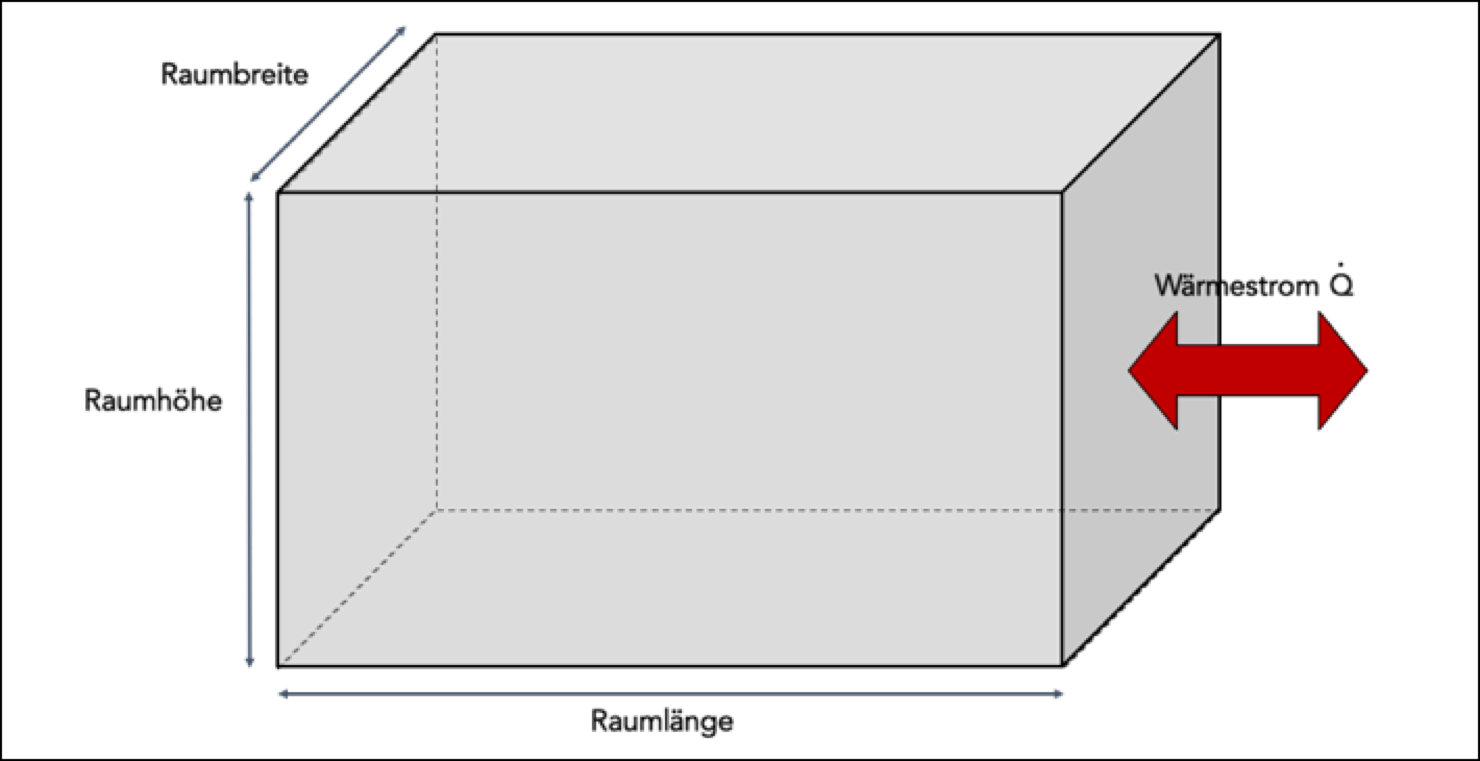
\includegraphics[width=\textwidth]{abbildungen/20160316_grundraum}
\caption{Grundmodell eines Raumes}
\label{fig:grundraum}
\end{figure}

Ausgehend von einer initialen Raumtemperatur und der externen Steuergröße der Umgebungslufttemperatur, wird zur Bestimmung der Temperatur innerhalb eines Raumes der Ausgleichsprozess zwischen Raum und Umgebung untersucht. Konkret muss dafür der ausgetauschte Wärmestrom näher betrachtet werden. Um diesen nach \ref{eq:qdot} zu berechnen, müssen zunächst die verschiedene modellrelevanten Eigenschaften des Raumes durch physikalische Parameter beschrieben werden. Für die Berechnung der Austauschoberfläche müssen die Raumbreite, -länge und -höhe bekannt sein. Außerdem sind der U-Wert einer Betonwand und die spezifische Wärmekapazität sowie die Dichte von Luft für die Bestimmung des Wärmestroms relevant.
Diese modellrelevanten Eigenschaften sind allesamt mit ihren Zahlenwerten in \ref{tab:eigenschaften_raum} zusammengefasst.

\begin{table}[H]
\centering
\small
\renewcommand{\arraystretch}{1.3}
\begin{threeparttable}
\begin{tabularx}{1\textwidth}{p{0.5\textwidth}m{0.2\textwidth}m{0.18\textwidth}}
\toprule
\textbf{Modellrelevante Eigenschaften} & \textbf{Wert} & \textbf{Einheit} \\
\cmidrule[0.5pt](r{0.25em}){1-1} 
\cmidrule[0.5pt](l{0.25em}){2-2}
\cmidrule[0.5pt](l{0.25em}){3-3}

Raumbreite & 7,81\tnote{1)} & $[m]$ \\ 
\ccol Raumlänge & \ccol 5,78\tnote{1)} & \ccol $[m]$ \\
Raumhöhe & 2,99\tnote{1)} & $[m]$ \\
\ccol Wärmedurchgangskoeffizient Betonwand & \ccol 1,0\tnote{2)} & \ccol $[\frac{W}{m^{2}*K}]$\\
Spezifische Wärmekapazität von Luft & 1.000,0\tnote{3)} & $[\frac{J}{kg*K}]$\\
\ccol Dichte von Luft & \ccol 1,25 \tnote{3)} & \ccol $[\frac{kg}{m^{3}}]$\\
\bottomrule
\end{tabularx}
\begin{tablenotes}[]\footnotesize\singlespacing\setlength\labelsep{0pt}
\item[1)] Werte durch eigene Vermessung des Raumes K004b vom 07.12.2015.
\item[2)] Schätzwert, geschätzt nach \cite[S.~409]{re14} mit Richtwerten aus \cite[S.~194ff.]{re14}.
\item[3)] Tabellenwert, entnommen aus \cite[S.~68]{ha13}.
\end{tablenotes}
\end{threeparttable}
\caption{Eigenschaften des einfachen Raummodells}
\label{tab:eigenschaften_raum}
\end{table}

Erfolgt die Bilanzierung des Raumes mithilfe des ersten Hauptsatzes der Thermodynamik nach \ref{eq:hauptsatz} und die Berechnung der inneren Energie nach \ref{eq:innereenergie}, so ergibt sich das folgende Gleichungssystem zur Bestimmung der Raumtemperatur. Das Grundmodell in Modelica hängt lediglich von der Steuergröße Außentemperatur ab:

\begin{lstlisting}[language=Modelica,caption={Einfaches Gleichungssystem des Raumgrundmodell in Modelica}, label=lst:grundraum]
equation
   /* calculate room volume */
   room_volume = room_length * room_height * room_breadth;
   /* calculate room mass */
   room_mass = room_volume * rho_air;
   /* calculate surface of heat exchange */
   exchange_surface = 2 * (room_length * room_breadth) + 2 * (room_length * room_height) + 2 * (room_breadth * room_height);
   /* calculate inner energy*/
   room_u = room_mass * cp_air * room_temperature;
   /* calculate derivative of the inner energy */
   der(room_u) = environment_qdot;
   /* calculate heatflow between room and environment */
   environment_qdot = u_wall * exchange_surface * (environment_temperature - room_temperature);
\end{lstlisting}

Damit ist ein Grundmodell für die Berechnung der Temperatur eines Raumes aufgestellt, wie es in \ref{fig:grundraum} graphisch zu sehen ist. Dieses wird im nächsten Schritt an die reale Einsatzumgebung angepasst.


\subsection{Modellerweiterung durch Berücksichtigung der realen Umgebung}

Im nächsten Schritt wird das einfache Raummodell zunächst an die reale Umgebung des Raumes K004b angepasst. Die Lage von K00b ist in \ref{fig:skizzek004a} ersichtlich. Es lässt sich erkennen, dass der Raum zwei Außenwände besitzt, die an Umgebungsluft grenzen. Zu diesen zählen die Wände Richtung Süden und Westen. Die anderen beiden Wände sowie die Decke und der Boden grenzen an weitere Gebäudeteile des K~Gebäudes. Der Raum im Modell bildet nach wie vor ein geschlossenes System. Zusammen mit dem K~Gebäude und der Umgebungsluft kann er als ein abgeschlossenes System angesehen werden, bei dessen Betrachtung potenzielle Wärmeströme zwischen Raum und Außenumgebung sowie Raum und K~Gebäude berücksichtigt werden müssen. Da die fließenden Wärmeströme im Vergleich zur sehr großen Energie innerhalb des K~Gebäudes und der Umgebung nur verschwindend gering sind, wird der Einfluss der Wärmeströme auf die beiden, den Raum umgebenden Teilsysteme vernachlässigt. Daher kann von konstanten und homogenen Temperaturen der beiden Teilsysteme ausgegangen werden.

Durch diese Erweiterung des Modells hängt die Raumtemperatur nun von zwei Wärmeströmen und damit indirekt von zwei externen Steuergrößen, der Temperatur der Umgebung und des K~Gebäudes, ab. Die Oberfläche des Raumes wird in die Austauschoberfläche mit der Umgebung und die mit dem K~Gebäude aufgeteilt, um die Wärmeströme separat berechnen zu können. Die Temperatur der Außenumgebung und die umgebenden des K~Gebäudes werden im Modell in Form von externe Steuergrößen berücksichtigt. Durch diese Festlegung erweitert sich das Gleichungssystem des Grundmodells in \ref{lst:grundraum} folgendermaßen:
\begin{lstlisting}[language=Modelica, caption={Erweitertes Gleichungssystem Modell des Raumes unter Berücksichtigung der realen Umgebung in Modelica}, label=lst:raumeins]
equation
   [...]
   /* calculate surface of heat exchange with the environment */
   environment_surface = room_length * room_height + room_breadth * room_height;
   /* calculate surface of heat exchange with the remaining building */
   building_surface = 2 * (room_length * room_breadth) + room_length * room_height + room_breadth * room_height;
   /* calculate derivative of the inner energy */
   der(room_u) = environment_qdot + building_qdot;
   /* calculate heatflow between room and environment */
   environment_qdot = u_wall * environment_surface * (environment_temperature - room_temperature);
   /* calculate heatflow between room and building */
   building_qdot = u_wall * building_surface * (building_temperature - room_temperature);
\end{lstlisting}

Damit wurde das Raummodell an die reale Umgebung angepasst und um die Temperatur innerhalb des Raumes zu bestimmen, wird nun neben der Ausgangstemperatur im Raum und der Umgebungstemperatur noch die Temperatur innerhalb des restlichen K~Gebäudes berücksichtigt. Im nächsten Schritt werden die realen, räumlichen Gegebenheiten im Modell abgebildet.


\subsection{Modellerweiterung durch Berücksichtigung der räumlichen Gegebenheiten}

Um das Modell an die realen Gegebenheiten des Raumes K004b anzupassen, müssen zwei bauliche Tatbestände beachtet werden. Wie sich aus \ref{fig:skizzek004a} entnehmen lässt, bildet eine Fensterfront die südlichen Außenwand des Raumes. Der U-Wert eines Fensters weicht erheblich von dem einer Wand ab, daher muss ein zusätzlicher Wärmestrom zwischen dem Raum und der Umgebung durch das Fenster im Modell berücksichtigt werden. Das Öffnen und Schließen der Fenster, mit den daraus resultieren Massenströmen, wird zunächst nicht explizit berücksichtigt, sodass  sich das Raummodell weiterhin als geschlossenes System betrachten lässt. 
Gleichermaßen wie das Fenster, soll der vorhandene Heizkörper zunächst in Form einer einfachen Wärmequelle in das Modell integriert werden. Durch den Heizkörper ist es möglich den Raum zu beheizen und somit eine Temperaturerhöhung im Raum herbeizuführen. Durch diese Anpassung des Modells erhöht sich die Anzahl der Steuergrößen erneut. 

Zur Beschreibung der Eigenschaften des Raummodells werden weitere physikalische Parameter notwendig. Dazu zählen der U-Wert einer Fensterscheibe sowie die Breite und Höhe der Fensterfront. Das Modell wird um die besagten Eigenschaften, die in \ref{tab:eigenschaften_raumerw} aufgelistet sind, ergänzt.

\begin{table}[H]
\centering
\small
\renewcommand{\arraystretch}{1.3}
\begin{threeparttable}
\begin{tabularx}{1\textwidth}{p{0.5\textwidth}m{0.2\textwidth}m{0.18\textwidth}}
\toprule
\textbf{Modellrelevante Eigenschaften} & \textbf{Wert} & \textbf{Einheit} \\
\cmidrule[0.5pt](r{0.25em}){1-1} 
\cmidrule[0.5pt](l{0.25em}){2-2}
\cmidrule[0.5pt](l{0.25em}){3-3}

Fensterbreite & 7,0\tnote{1)} & $[m]$ \\ 
\ccol Fensterhöhe & \ccol 2,08\tnote{1)} & \ccol $[m]$ \\
Wärmedurchgangskoeffizient Glas & 2,0\tnote{2)} & $[\frac{W}{m^{2}*K}]$\\

\bottomrule
\end{tabularx}
\begin{tablenotes}[]\footnotesize\singlespacing\setlength\labelsep{0pt}
\item[1)] Werte durch eigene Vermessung des Raumes K004b vom 07.12.2015.
\item[2)] Tabellenwert, geschätzt nach \cite[S.~270ff.]{h2000}.
\end{tablenotes}
\end{threeparttable}
\caption{Weitere Eigenschaften des Raummodells}
\label{tab:eigenschaften_raumerw}
\end{table}
 
Durch diese Anpassung verändert sich die Austauschoberfläche mit der Umgebung, die sich nun in zwei Flächen mit verschiedenen Wärmedurchgangskoeffizienten unterteilt. Des Weiteren wird eine Wärmequelle für die Heizung ergänzt, sodass sich folgende Änderungen des Gleichungssystems im Vergleich zum bisherigen Modell in \ref{lst:grundraum} ergeben:

\begin{lstlisting}[language=Modelica, caption={Erweitertes Gleichungssystem des Raumes unter Berücksichtigung der räumlichen Gegebenheiten in Modelica},label=lst:raumzwei]
equation
   [...]
   /* calculate surface of heat exchange with the environment */
   environment_surface = room_length * room_height + room_breadth * room_height - window-surface;
   /* calculate surface of heat exchange with the remaining building */
   building_surface = 2 * (room_length * room_breadth) + room_length * room_height + room_breadth * room_height;
   /* calculate surface of window with the environment */
   window_surface=(window_length*window_height);
   /* calculate derivative of the inner energy */
   der(room_u) = environment_qdot + building_qdot + window_qdot + radiator_qdot;
   /* calculate heatflow between room and environment through the walls */
   environment_qdot = u_wall * environment_surface * (environment_temperature - room_temperature);
   /* calculate heatflow between room and environment through the window */
   building_qdot = u_glass * window_surface * (environment_temperature - room_temperature);
   /* calculate heatflow between room and building */
   building_qdot = u_wall * building_surface * (building_temperature - room_temperature);
\end{lstlisting}

Das Modell berücksichtigt nun auch die räumlichen Gegebenheiten und beschreibt dadurch die realen Zusammenhänge in groben Zügen. Die bisher berücksichtigten Zusammenhänge des Modells sind in \ref{fig:raumeins} veranschaulicht. Ein Controller kann die Heizung jedoch nicht beliebig als Wärmequelle zur Steuerung der Raumtemperatur einsetzen. Daher wird im folgenden Abschnitt ein detaillierteres Modell des Heizkörpers entwickelt, um eine Steuerung des Heizkörpers durch den Controller zu ermöglichen. 

\begin{figure}
\centering
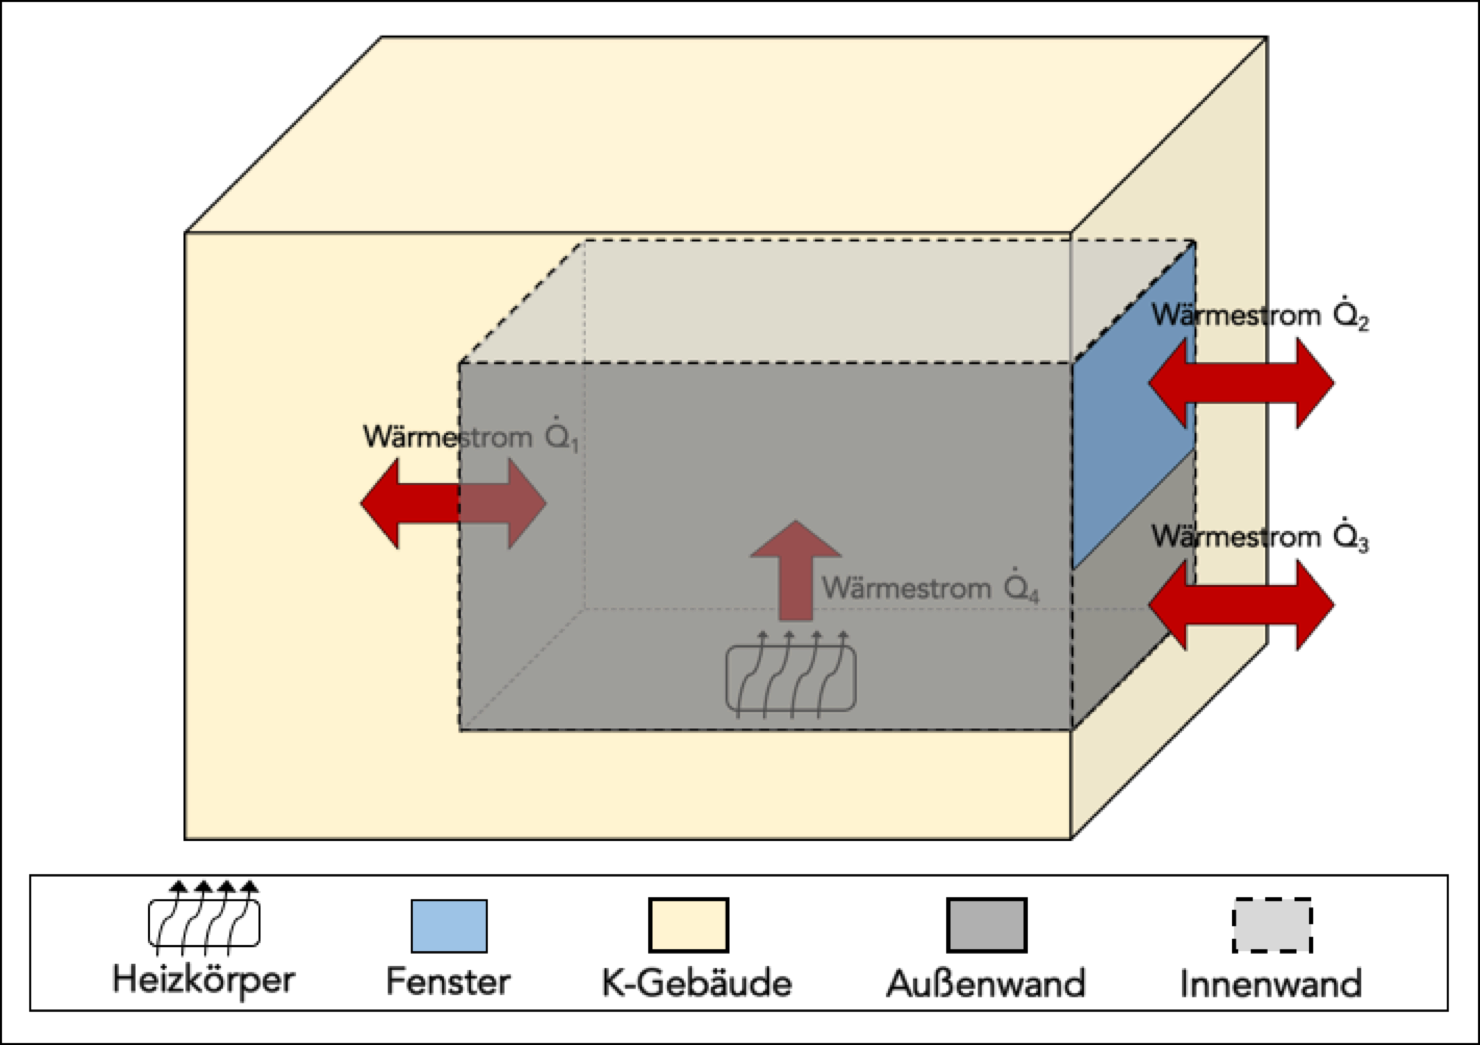
\includegraphics[width=\textwidth]{abbildungen/20160316_raumeins}
\caption{Erweitertes Raummodell}
\label{fig:raumeins}
\end{figure}



\subsection{Das Heizkörpermodell}

Der Heizkörper in Raum K004b lässt sich nach \cite[S.~824f.]{re14} als Stahlrohrradiator identifizieren. Er besteht aus genormten zweisäuligen Gliedern, die jeweils an einem Sammler oben und unten miteinander verschweißt den Heizkörper bilden. Dabei stellen die Temperatur am Einlass des Heizkörpers und der Massenstrom des Heizwassers zwei weitere Steuergrößen für das Modell dar. Die Temperatur am Einlass wird durch die Heizanlage vorgegeben, folglich ist sie eine externe Steuergröße. Der Massenstrom hingegen wird unmittelbar durch den Stellantrieb gesteuert. Er kann vom Controller genutzt werden, um Einfluss auf die Raumtemperatur zu nehmen. Daher stellt der Massenstrom eine veränderbare Steuergröße dar. Da der ins Modell einfließende Wärmestrom des Heizkörpers nicht linear von der Temperaturdifferenz des Heizwassers zur Raumtemperatur abhängt, erfolgt eine Diskretisierung des Heizkörpers in Volumenelemente. Dadurch soll eine adäquate Abbildung des Heizkörpers im Modell generiert werden. 

Durch eine Bilanzierung von jedem diskreten Volumenelement des Heizkörpers mithilfe des ersten Hauptsatzes der Thermodynamik nach \ref{eq:hauptsatz} wird eine Berechnung des einfließenden Wärmestroms ermöglicht. Der gesamte Wärmestrom berechnet sich anschließend aus der Summe der einzelnen Wärmestrome zwischen Raum und den Volumenelementen. Diese wiederum lassen sich wie folgt nach \ref{eq:qdot} berechnen. Bei der Diskretisierung wird mithilfe der Heizwassertemperatur am Einlass eines Volumenelements die Temperatur am Auslass berechnet und zusammen mit dem Massenstrom an das nächste Volumenelement weitergereicht.
Allerdings müssen für die Berechnung zunächst noch weitere Eigenschaften in das Raummodell aufgenommen werden, welche in \ref{tab:eigenschaften_heiz} abgebildet sind.

\begin{table}[H]
\centering
\small
\renewcommand{\arraystretch}{1.3}
\begin{threeparttable}
\begin{tabularx}{1\textwidth}{p{0.5\textwidth}m{0.2\textwidth}m{0.18\textwidth}}
\toprule
\textbf{Modellrelevante Eigenschaften} & \textbf{Wert} & \textbf{Einheit} \\
\cmidrule[0.5pt](r{0.25em}){1-1} 
\cmidrule[0.5pt](l{0.25em}){2-2}
\cmidrule[0.5pt](l{0.25em}){3-3}


Zahl der Glieder & 106\tnote{1)} & Stück \\ 
\ccol Säulen pro Glied & \ccol 2\tnote{1)} & \ccol Stück \\
Vertikaler Rohrdurchmesser & 0,0255\tnote{1)} & $[m]$\\
\ccol Horizontaler Rohrdurchmesser & 0,05 \ccol 2\tnote{1)} & \ccol $[m]$ \\
Höhe der Glieder & 0,4\tnote{1)} & $[m]$\\
\ccol Länge eines Glieds & 0,045 \ccol 2\tnote{2)} & \ccol $[m]$ \\
Wassermasse innerhalb eines Gliedes & 0,35\tnote{2)} & $[kg]$\\
\ccol Spezifische Wärmekapazität von Wasser &\ccol 4.200,0\tnote{4)} &\ccol $[\frac{J}{kg*K}]$\\
Wärmedurchgangskoeffizient Heizkörper & 16\tnote{3)} & $[\frac{W}{m^{2}*K}]$\\
\ccol Anzahl Volumenelemente & \ccol 10&\ccol  Stück\\

\bottomrule
\end{tabularx}
\begin{tablenotes}[]\footnotesize\singlespacing\setlength\labelsep{0pt}
\item[1)] Wert aus eigener Vermessung des Raumes K004b vom 07.12.2015.
\item[2)] Tabellenwert, entnommen aus \cite[S.~825]{re14}.
\item[3)] Tabellenwert, geschätzt nach \cite[S.~191ff.]{re14}.
\item[4)] Tabellenwert, entnommen aus \cite[S.~619]{ba12}.
\end{tablenotes}
\end{threeparttable}
\caption{Eigenschaften des Heizkörpermodells}
\label{tab:eigenschaften_heiz}
\end{table}

Die Eigenschaften des realen Heizkörpers werden zunächst im Modell abgebildet und anschließend zentral auf die diskretisierten Volumenelemente umgerechnet, wie in Listing \ref{lst:heiz} ab Zeile 18 zu sehen ist. Dazu gehört die Zahl und die Wassermasse der Glieder, die Höhe des Heizkörpers sowie Anzahl, Durchmesser und Längen der verschiedenen Rohre. All diese Eigenschaften werden benötigt, um die Wärmeaustauschoberfläche zu bestimmen. Die spezifische Wärmekapazität des Heizwassers und der Wärmedurchgangskoeffizient des Heizkörpers müssen bekannt sein, um letztendlich auf die Wärmestrome der einzelnen diskreten Volumenelemente des Heizkörpers schließen zu können.

\lstinputlisting[language=Modelica ,caption={Auszüge des Modelica Modells vom Heizkörper in K004b}, label=lst:heiz, linerange={20-20, 47-57,58-60, 106-120}]{listings/room_model_listing.mo}

Das Modell des Heizkörpers ist als Subkomponente in das Raummodell integriert. Durch das Modell des Heizkörpers wird ein physikalisch motivierter, mittelbarer Zusammenhang zwischen der Heizleistung und dem Massenstrom hergestellt, welcher insbesondere von einem modellprädiktiv regelnden Controller genutzt werden kann.

Schon bei den Einsatzzielen der Anlage in Abschnitt\ref{sec:anforderungen} war gefordert, den Zusammenhang zwischen der Sonneneinstrahlung und der Raumtemperatur zu untersuchen und dabei Störgrößen explizit in Kauf zu nehmen. In einem nächsten Erweiterungsschritt wird das Raummodell an weitere reale Gegebenheiten angepasst. Daher erscheint es passend, das die Fensterfront in Richtung Süden ausgerichtet ist, wodurch die Sonneneinstrahlung eine Wirkung auf die Raumtemperatur besitzt. Außerdem kann die Nutzung des Raumes als Büro für wissenschaftliche Mitarbeiter als eine Störgröße betrachtet werden.

\subsection{Modellerweiterung durch Berücksichtigung der Sonneneinstrahlung und der Störgrößen}
\label{sub:modsonne}

Der Raum K004b wird regulär als Büro genutzt, weshalb verschiedene Faktoren als Störgrößen in Bezug auf die Raumtemperatur in Betracht kommen. Zum einen wird durch die Menschen und deren Rechner Wärme in den Raum eingebracht und zum anderen werden Fenster und Türen in unregelmäßigen Abständen immer wieder geöffnet und geschlossen. Dabei werden Massenströme zwischen Raum, Außenumgebung sowie K~Gebäude ausgetauscht, welche jedoch zunächst nicht modelliert werden sollen. Stattdessen sollen diese als Störgröße betrachtet werden, die es durch die Modellprädiktive Regelung auszugleichen gilt. Die abgestrahlte Wärme von Rechnern und Menschen werden als einfache Wärmequelle im Modell berücksichtigt. 

Die auf die südseitige Fensterfront treffende Sonnenstrahlung, bringt ebenfalls einen Wärmestrom in den Raum ein und hat Auswirkungen auf die herrschende Raumtemperatur. Die Sonneneinstrahlung  wird im Modell zunächst als eine einfache Wärmequelle aufgefasst.
Beide Erweiterungen stellen äußere Steuergrößen dar, die weder von der Anlage, noch dem Modell beeinflusst werden können. Das Raummodell erweitert sich wie folgt:

\begin{lstlisting}[language=Modelica, caption={Erweitertes Gleichungssystem des Raummodells unter Berücksichtigung der Sonneneinstrahlung und weiterer Störgrößen},label=lst:raumdrei]
equation
   [...]
   /* calculate derivative of the inner energy */
   der(room_u) = environment_qdot + building_qdot + window_qdot + radiator_qdot + sun_qdot + otherfactors_qdot;
\end{lstlisting}

\begin{figure}
\centering
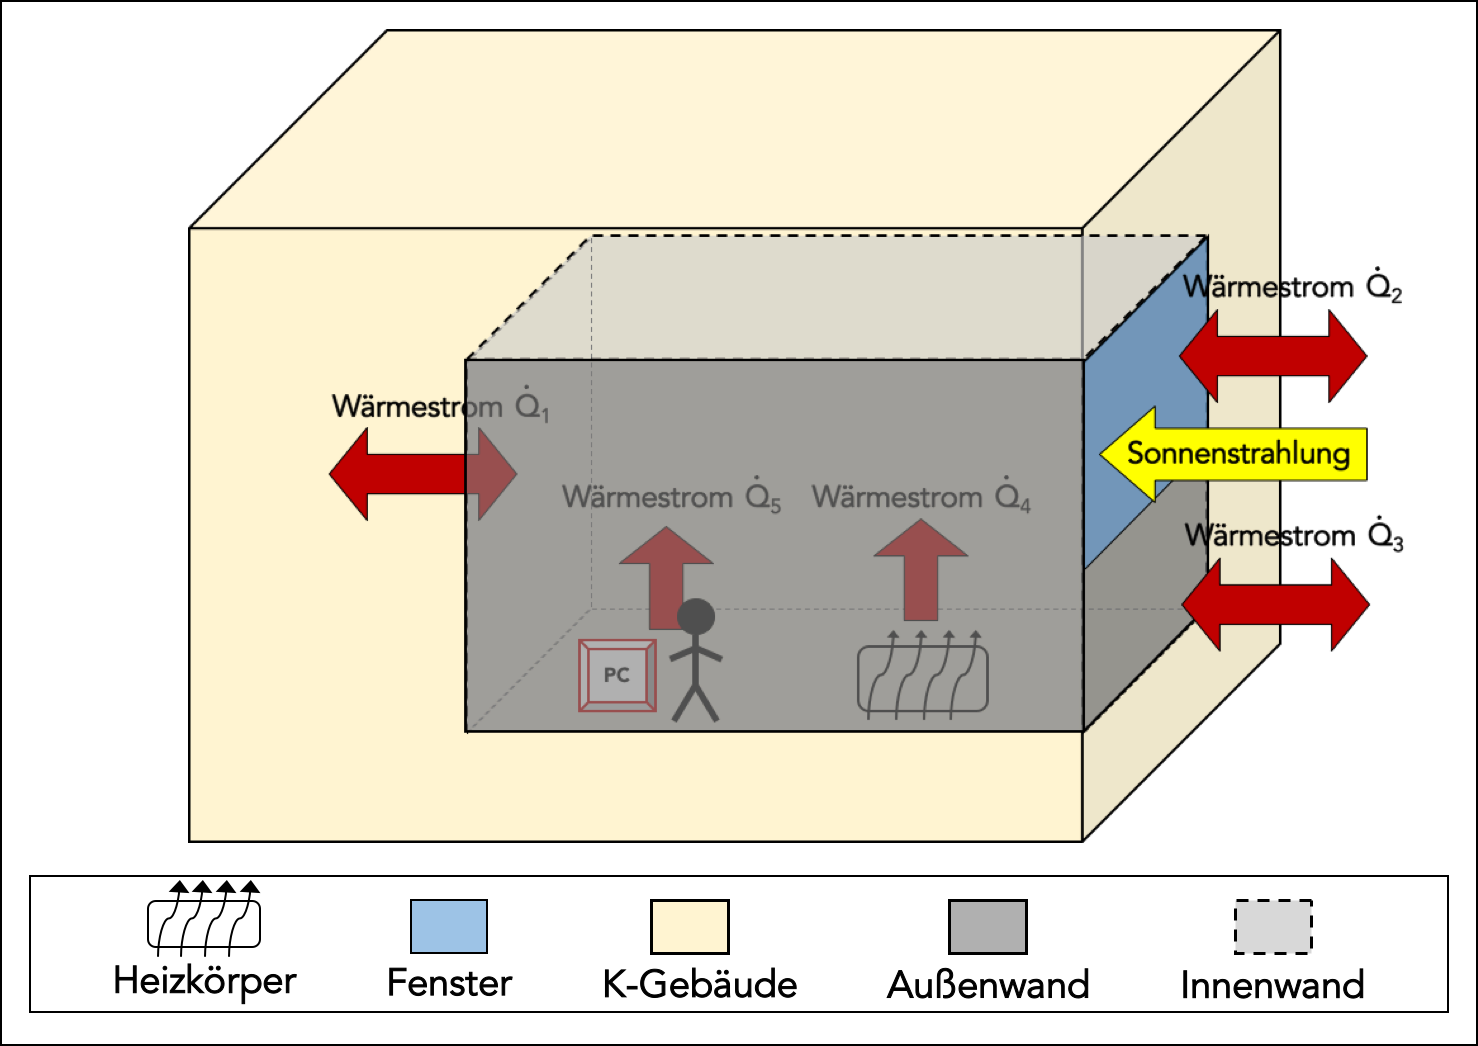
\includegraphics[width=\textwidth]{abbildungen/20160317_raumzwei}
\caption{Erweitertes Raummodell}
\label{fig:raumdrei}
\end{figure}


Die Zusammenhänge des erweiterten Modells lassen sich, wie in \ref{fig:raumdrei} gezeigt, visualisieren. Der Einfluss der Sonnenstrahlung wurde bereits in Kapitel \ref{sub:sonne} näher erläutert. Er wird nun an die realen Gegebenheiten des Raumes K004b angepasst. Als Messwerte stehen Werte der Globalstrahlung zur Verfügung, welche für eine Berücksichtigung im Modell in die effektive Strahlungsintensität an der Fensterfront umgerechnet werden müssen.

Zur Berechnung der effektiven Strahlungsintensität müssen neben der Globalstrahlung auch der Azimut und Höhenwinkel der Sonne bekannt sein, wodurch sich die Komplexität der Berechnungen erhöht. Um jedoch die Komplexität des Modells zu schonen, werden die Effektivwerte der Sonnenstrahlung von einem Python Skript berechnet und anschließend dem Modell übergeben. Zudem hat dieses Vorgehen den Vorteil, dass im \textit{pysolar} Package \cite{pysolar} bereits der relativ exakte Algorithmus nach \cite{re08} implementiert ist. 
Das Skript zur Konvertierung ist in Listing \ref{lst:sonne} dargestellt. 
Zur Berechnung des Azimut- und Sonnenhöhenwinkels wird der Längen- und Breitengrad des K~Gebäudes sowie die Höhe über dem Meeresspiegel benötigt. Zudem muss die Ausrichtung der Fensterfläche bekannt sein, um auf die effektive Solarstrahlung zu schließen zu können. Eine ausführliche Beschreibung zur Sonnenlaufbahn und deren Berechnung finden sich bei \cite{qu11} und \cite{ka13}. Die Werte hiervon wurden mithilfe von \cite{go15} ermittelt und sind in Listing \ref{lst:sonne} in Zeile sieben bis zehn zu finden.

\lstinputlisting[language=Python ,caption={Programm zur Umrechnung der Globalstrahlung in die effektive Solarstrahlung an der Fensterfront am Raum K004b}, label=lst:sonne]{listings/radiation_conversion_k004b.py}

Außerdem wird der Startzeitpunkt und der Abstand zwischen den einzelnen Messpunkten der Globalstrahlung benötigt, da der Stand der Sonne von der Uhrzeit abhängt. Nach dem Einlesen der Messdaten aus der Datei globalstrahlung.csv wird anschließend für jeden einzelnen Messwert und -zeitpunkt der Azimut und Sonnenhöhenwinkel berechnet. Darauf basierend wird geprüft, ob die Sonne senkrecht am Himmel steht, noch nicht aufgegangen ist oder die Fläche im Schatten liegt. Ist dies der Fall, trifft keine effektive Strahlung auf das Fenster. Für niedrige Sonnenstände würden sich sehr hohe und unrealistische effektive Strahlungswerte ergeben. Daher sind diese für kleinere Winkel des Sonnenstandes als fünf Grad begrenzt.

Ansonsten wird der effektive Strahlungswert nach \cite[S.~67f.]{qu11} berechnet und in der Datei qdotsun-effective gespeichert. Dieses Programm findet in leicht abgewandelter Form einfach zur Umrechnung einzelner Messwerte Verwendung, indem das Einlesen und Speichern der umgerechneten Daten durch die Abfrage eines Messwertes und die Übergabe einer Variable durch einen umgerechneten Messwert ersetzt wird.

Der effektive Strahlungswert wird durch den Transmissionsgrad des Fensterglases weiter abgeschwächt. Dieser wird durch einen weiteren Parameter, dem $window\_transmission$, beschrieben. Der Schätzwert für die doppelscheibige Verglasung des Fensters in K004b stammt aus \cite[S.~63]{ha13}. Dadurch erweitert sich das Modell um ein Fenster als Subkomponente:

\begin{lstlisting}[language=Modelica, caption={Fenster als Subkomponente des Raummodells},label=lst:raumdrei]
model Window
	Modelica.SIunits.DensityOfHeatFlowRate qdotsun_effective;
	Modelica.SIunits.HeatFlowRate qdot_effective;
	parameter Real window_transmission = 0.5;
	Modelica.SIunits.Area window_surface;
  equation
  	qdot_effective = qdotsun_effective * window_transmission * window_surface;
end Window;
\end{lstlisting}

Das Modell zum jetzigen Zeitpunkt berücksichtigt alle relevanten Einflüsse und die physikalische Effekte, die damit einhergehen. Die Modellkomplexität ist noch überschaubar. Die Modellbildung ist hiermit, mit einer noch überschaubaren Modellkomplexität, abgeschlossen. Eine Übersicht des gesamten Raummodells findet sich im Anhang \ref{att:raummod}. Bei der Modellbildung wurde auf eine Programmierung mit einer klaren Struktur wert gelegt. Daher sind die Variablen der Modelle strikt nach Parametern, Controls und Zuständen gegliedert.

Das Schaltbild in \textsc{Dymola}, welches als Umgebung zur Modellbildung und Simulation genutzt wurde, ist in \ref{fig:raumdym} abgebildet. Auf diesem wird deutlich, dass das Modell insgesamt sechs verschiedene Steuergrößen und damit Freiheitsgrade besitzt. Fünf dieser Steuergrößen sind durch äußere Bedingungen festgelegt: durch die Außentemperatur, die Temperatur im K~Gebäude, die Temperatur am Einlass der Heizung, die anderen Faktoren sowie die Solarstrahlung. Folglich kann der Controller lediglich den Massenstrom des Heizwassers zur Beeinflussung der Raumtemperatur nutzen, um auf Änderungen der fünf äußeren Steuergrößen zu reagieren. 

\begin{figure}
\centering
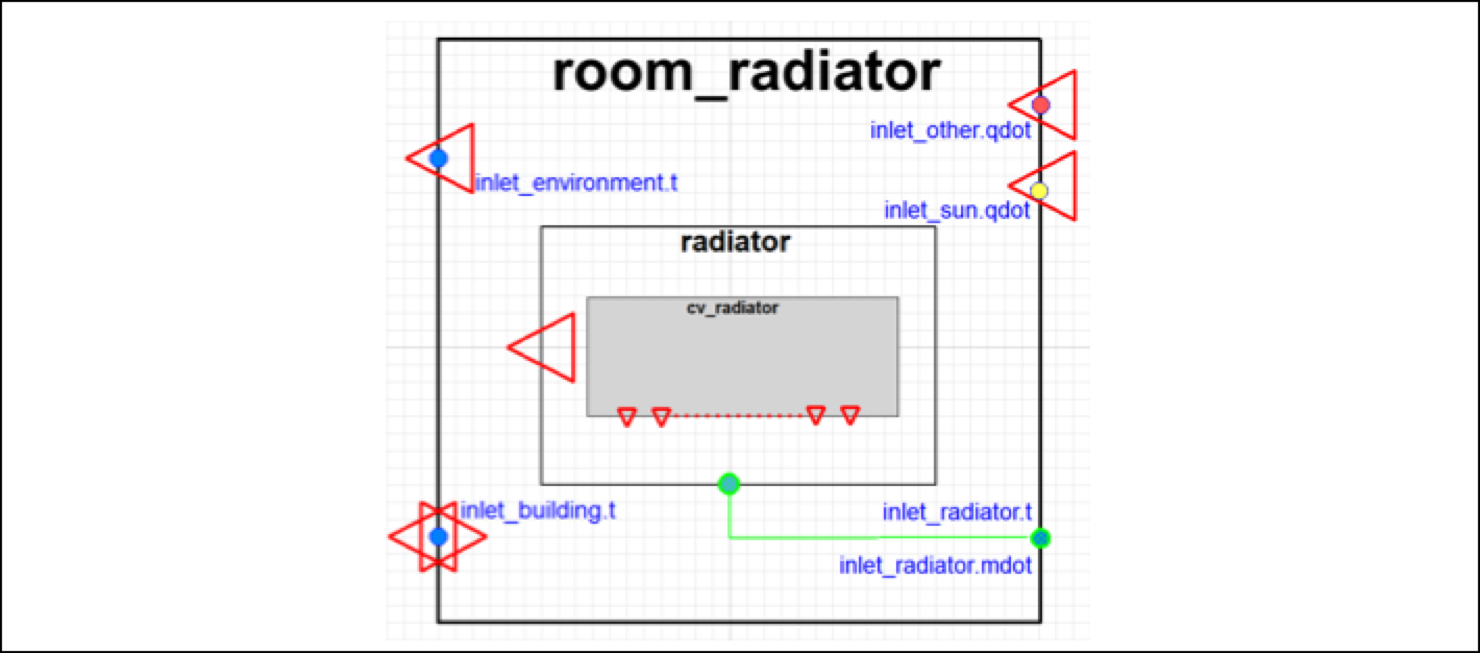
\includegraphics[width=\textwidth]{abbildungen/20160331_raumdym}
\caption{Schaltbild des Raummodells in Dymola}
\label{fig:raumdym}
\end{figure}

Es gibt weitere Effekte innerhalb des Raumes K004b, die jedoch bewusst nicht berücksichtigt werden. Zu diesen zählt unter anderem die Energie innerhalb der Wände und des Mobiliars, welche bei einer abrupten Abkühlung der Raumlufttemperatur einen stark erwärmenden Einfluss durch die Abstrahlung von Wärme besitzt. Dieses Phänomen ist in Kapitel \ref{chap:theoretischegrundlagen} beschrieben und wird als Wärmekonvektion bezeichnet. Da eine solch starke Abkühlung der Raumluft jedoch nur über einen längeren Zeithorizont entstehen kann, würde dieser ein Modellprädiktiver Controller unmittelbar gegensteuern. Dadurch wird dieser Effekt als Störgröße wahrgenommen, die durch eine Modellprädiktive Regelung ausgeglichen wird.


\section{Simulation und Modellanpassung}

In diesem Abschnitt erfolgt zunächst die Simulation der Raumtemperatur unter Verwendung des Modells. Dazu werden für die Steuergrößen reale Messwerte vorgegeben, um die Güte des Modells abzuschätzen zu können, durch einen Vergleich der berechneten und tatsächlichen gemessen Werte. Abschließend erfolgt eine Anpassung der Modellparameter mit Hilfe von \cite{casiopeia}, um die Modellgüte zu verbessern.

\subsection{Simulation und Validierung des Modells}

Die Validierung des Modells unterteilt sich in zwei Schritte. Zunächst wird das Raummodell ohne die Verwendung des Heizkörpers simuliert. Auf diese Weise soll überprüft werden, ob in dem Grundmodell alle wichtigen physikalischen Effekte berücksichtigt wurden. Im nächsten Schritt erfolgt eine Simulation, bei der der Heizkörper zum Einsatz kommt. Mithilfe  dieses Simulationsdurchgangs soll die Güte des Heizkörpermodells ermittelt werden.
Für die ersten Simulation gilt es ein Zeitintervall zu finden, welches eine möglichst lange Dauer vorweist, während dem wenige Störfaktoren aufgetreten sind und der Heizkörper möglichst nicht genutzt wurde. Ein solches Zeitintervall findet sich über die Weihnachtsfeiertage vom 23.12.2105 bis zum 28.12.2015, da aufgrund der Feiertage das Büro nicht genutzt wurde.
Das Intervall umfasst etwas mehr als fünf Tage, wobei an den ersten Tagen relativ milde Außentemperaturen zwischen $8^{\circ}C$ und $16^{\circ}C$ geherrscht haben. Erst am letzten Tag nähert sich die Außenlufttemperatur dem Gefrierpunkt von $0^{\circ}C$. Die Sonne hat an jedem der betrachteten Tage gegen Mittag geschienen und den Raum dadurch erwärmt.
Die genauen Messdaten der Globalstrahlung und Außentemperatur für diesen Zeitraum, zwischen denen jeweils zehnminütige Intervalle liegen, wurden von \cite{wetter} zur Verfügung gestellt. Sie sind in REFXXXXBILD veranschaulicht sowie auf der angehängten CD in der Datei XXXXXX zu finden.
Der Simulation wurde außerdem eine Temperatur von $22^{\circ}C$ im Inneren des K~Gebäudes und die gemessene Initialtemperatur von $22,8^{\circ}C$ zugrunde gelegt. In \ref{fig:valid1} sind die Ergebnisse der Simulation im Plot abgebildet. Die Simulationsergebnisse  werden im Folgenden analysiert.


\begin{figure}
\centering
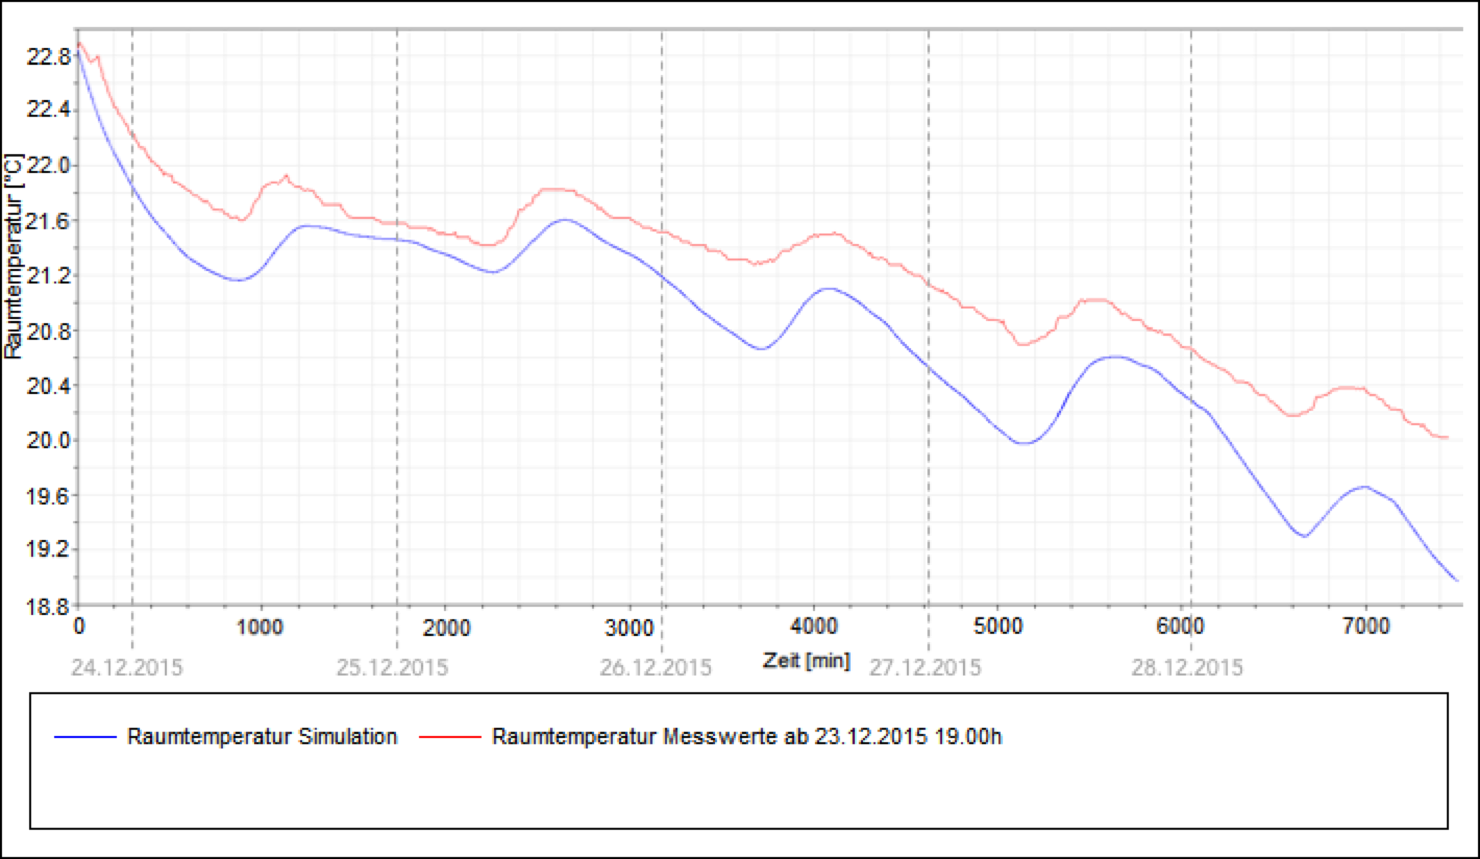
\includegraphics[width=\textwidth]{abbildungen/20160328_validierung1}
\caption{Simulation des Raummodells ohne Einsatz der Heizung}
\label{fig:valid1}
\end{figure}

Die Skalierung der Abszisse ist in Minutenschritte eingeteilt. Insgesamt erstreckt sich die Simulation über einen Zeitraum von 7500 Minuten. Im Rahmen der Modellprädiktiven Regelung werden üblicherweise deutlich kürzere Simulationszeiträume betrachtet. Da hier jedoch in erster Linie ein Abgleich des Modells mit der Realität erfolgen soll, wurde eine längere Periode gewählt.

Auf den ersten Blick lässt sich bereits erkennen, dass die simulierte Temperaturkurve eine ähnliche Dynamik wie der gemessene Temperaturverlauf aufweist. Von Beginn der Simulation bis hin zum 26.02.2016 stimmt das Systemverhalten sehr gut mit der Realität überein. Von dort an bis zum Ende des Simulationszeitraums knickt die simulierte Kurve leicht ab. 
Außerdem lässt sich eine minimale zeitliche Verzögerung des Modells zur Realität erkennen, die auf eine gewisse Trägheit des Modells gegenüber der Realität hindeutet.
Die simulierte Temperaturkurve liegt während des gesamten Intervalls unterhalb der Messwerte. Ursache hierfür könnte ein zu hoher Wärmeverlust im Modell sein.  
Im Temperaturverlauf lässt sich der Einfluss der Solarstrahlung auf die Raumtemperatur deutlich erkennen. Die periodischen Schwankungen, die einen täglichen Temperaturanstieg zur Mittagszeit bis in den späten Nachmittag zeigen, sind durch den Einfall der Sonnenstrahlen in den Raum begründet. 

Insgesamt ist hervorzuheben, dass die simulierte von der tatsächlich gemessenen Temperatur innerhalb der ersten beiden Tage um nicht mehr als $0,4^{\circ}C$ und während der gesamten Simulationsdauer um nicht mehr als $1^{\circ}C$ abweicht.
Die Messabweichung des Webthermographs liegt bei $\pm 0,26^{\circ}C$ , die der beiden RTM1 Temperaturfühler hingegen bei $\pm 0,5^{\circ}C$.
Die Messwerte der Wetterstation auf dem Physikhochhaus des Karlsruher Instituts für Technologie haben eine zehnminütige Auflösung, wohingegen die Raumtemperatur minütlich aufgezeichnet wurde.
Durch die örtliche Trennung von 1km Luftlinie zwischen der Messstation und dem K~Gebäude, ist es durchaus möglich, dass es zu Abweichungen zwischen den Messwerten und der effektiven Strahlung am Raum aufgrund unterschiedlicher lokaler Bewölkung kommt. 

Im Rahmen der Modellprädiktiven Regelung werden wie bereits erwähnt kürzere Simulationszeiträume im unteren Stunden- beziehungsweise höheren Minutenbereich betrachtet, weshalb die Güte des Modells ohne den Einsatz des Heizkörpers dazu ausreichend ist.

Im nächsten Schritt findet eine Simulation mit dem Einsatz des Heizkörpers statt, um das vollständige Modell mit der Realität abzugleichen. Der Heizkörper wurde für die folgende Modellsimulation in insgesamt vier Volumenelemente diskretisiert.
Nun musste ein Zeitintervall gefunden werden, indem die Raumtemperatur unter die untere Schalttemperatur von $20^{\circ}C$ fällt, sodass der Heizkörper zum Erwärmen des Raumes bis zum oberen Schaltpunkt von $21,5^{\circ}C$ genutzt wird und  schließlich die Raumluft das Heizkörperventil wieder abkühlt. Ein geeignetes Intervall findet sich vom 28.12.2015 bis zum 30.12.2015. Dieses ist zudem gut geeignet, da das Büro innerhalb dieses Zeitraums nicht genutzt wurde und dadurch keine weiteren Störgrößen in der Betrachtung auftreten.
Die Messdaten für die Globalstrahlung und Außenlufttemperatur wurden auch für diese Simulation in zehnminütigen Intervallen von \cite{wetter} zur Verfügung gestellt und sind auf der angehängten CD in der Datei XXXXXXXXXXXX zu finden. Am Nachmittag des 29.12.2016 hat die Sonne leicht geschienen. Die Außenlufttemperatur hat sich leicht unterhalb des Gefrierpunkts bis hin zu 6 Grad bewegt. Der Heizkörper wurde am Nachmittag des 29.12.2015 bis abends genutzt.
Wie auch bei der voragehenden Simulation, wurden hier eine Temperatur von $22^{\circ}C$ im K~Gebäude und die gemessene Initialtemperatur von $21,25^{\circ}C$ zugrunde gelegt. Die Simulationsergebnisse sind im Plot \ref{fig:valid2} abgebildet und werden wiederum im Folgenden analysiert.

\begin{figure}
\centering
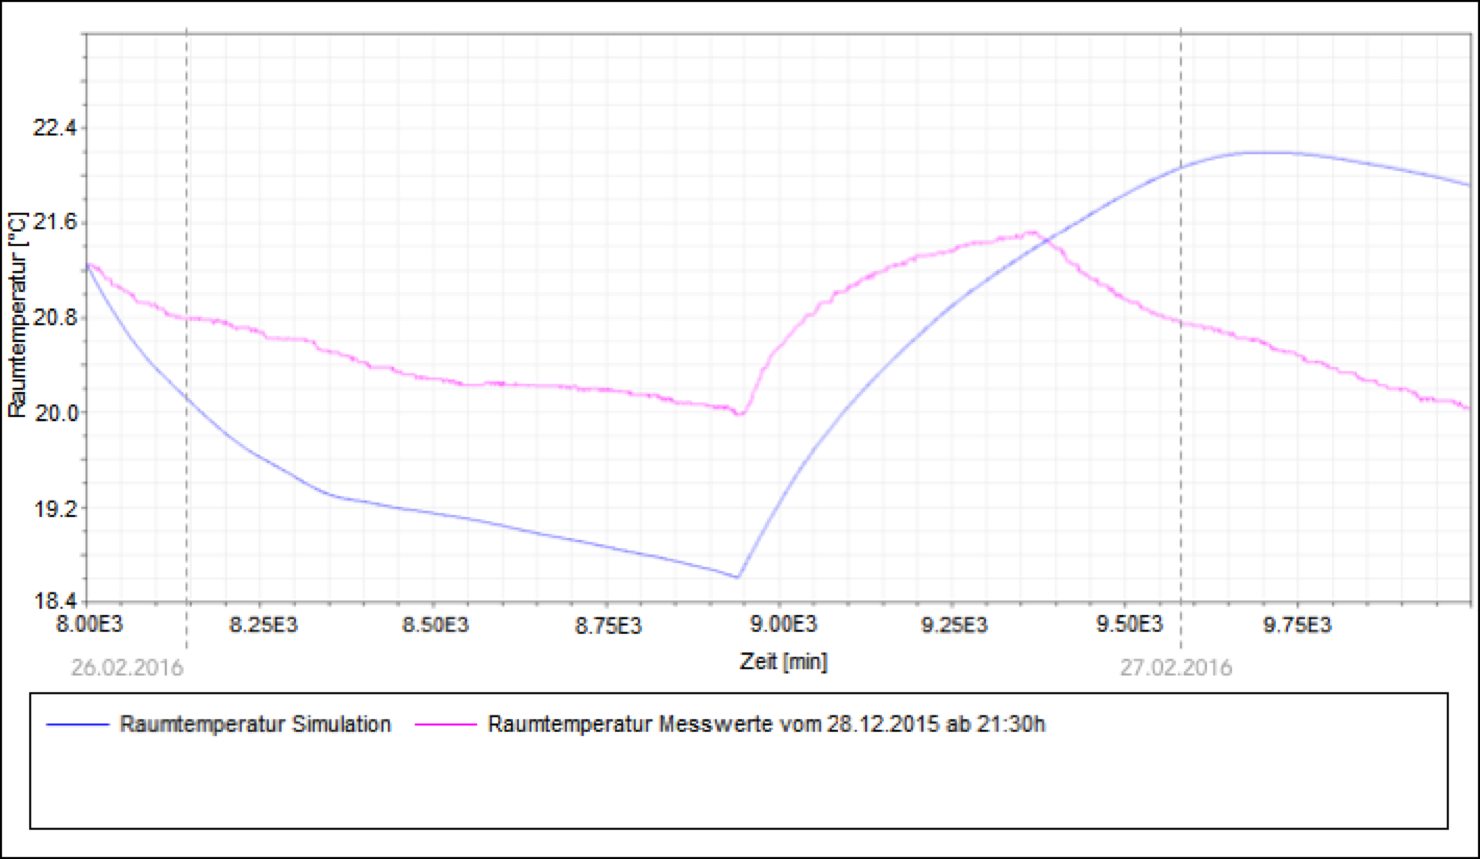
\includegraphics[width=\textwidth]{abbildungen/20160328_validierung2}
\caption{Simulation des Raummodells mit dem Einsatz des Heizkörpers}
\label{fig:valid2}
\end{figure}

Der Simulationszeitraum beginnt am Abend des 28.02.2015 und erstreckt sich über insgesamt 2000 Minuten bis zum frühen Morgen des 30.12.2015. Die Simulationsergebnisse bestätigen die Ergebnisse, der vorherigen Simulation, da sich auch hier eine schnellere Abkühlung des Raummodells als im reale Raum beobachten lässt. Dies liefert einen Hinweis auf einen zu hohen Wärmeverlust im Modell.
Die Systemdynamik des Modells folgt in etwa der Realität bis der Heizkörper nach etwa 950 simulierten Minuten eingeschaltet wird. 
Das Öffnen des Heizkörperventils ist sowohl im Modell, als auch in den Messwerten sehr gut zu sehen, da es einen signifikanten Anstieg der Raumtemperatur herbeiführt. Es wird deutlich, dass die Modellreaktion gleichzeitig einsetzt, jedoch deutlich langsamer abläuft als in der Realität. Außerdem wird im Modell weitaus mehr Wärme in den Raum eingebracht als in der Realität, was auf eine erhöhte Wärmezufuhr entweder durch den Heizkörper oder durch die Solarstrahlung hinweist. Wie zuvor erwähnt könnte die lokale Bewölkung eine Ursache hierfür sein.
Die beobachtete Trägheit des Modells kann auf eine unzureichende Diskretisierung hinweisen, weshalb die Anzahl der Volumenelemente innerhalb des Modells auf zehn erhöht wurde. Die anschließenden Untersuchungen zeigen, dass die Modellgüte durch die erhöhte Diskretisierung gesteigert wird.

Insbesondere im Zusammenhang mit den zuvor festgestellten Unsicherheiten bei den Messwerten lässt sich feststellen, dass die Simulationskurve die Dynamik des realen Systems erkennbar widerspiegelt, wenn auch mit einer gewissen Trägheit verbunden.

Zusammenfassend lässt sich festhalten, dass das Modell trotz gewisser Abweichungen die grundlegende Systemdynamik der Realität beschreibt. Dies wurde insbesondere durch die langen Simulationsintervalle deutlich, die für den späteren Einsatz des Modells keine weiterer Relevanz haben.

Um die Modellgüte hinsichtlich des Einsatzes der Heizung zu verbessern, wird im Folgenden eine Parameterschätzung vorgenommen. Abschließend wird überprüft, ob das Modell den Anforderungen für eine Modellprädiktive Regelung mit \textsc{JModelica.org} genügt.


\subsection{Anpassung des Modells}

Ziel des Abschnittes ist eine Verbesserung des Raummodells, welche durch eine Parameterschätzung mit \cite{casiopeia}, einer freien Softwareumgebung für die optimale Versuchsplanung und Parameterschätzung, durchgeführt wird.
Wie bereits erwähnt, werden beim Einsatz des Modells mit Modellprädiktiver Regelung kürzere Intervalle betrachtet, daher erfolgt die weitere Modelloptimierung anhand von kürzeren Intervallen. Die Parameterschätzung wurde mit freundlicher Unterstützung von Herrn \textsc{Adrian Bürger} durchgeführt, der das Übersetzen des Modell und die Ausführung übernommen hat.

Die Parameterschätzung erfolgt systematisch, um die einzelnen Modellparameter anzupassen. Der Wärmedurchgangskoeffizient der Raumwände und des Heizkörpers sowie der Transmissionsgrad der Fensterscheiben sollen als Parameter geschätzt werden. Die Schätzung erfolgt in drei Schritten. Der Wärmedurchgangskoeffizient der Glasscheibe wird als fester Wert angenommen, da sich aufgrund der offensichtlichen Korrelation zwischen den beiden Wärmedurchgangskoeffizienten voneinander nicht-physikalische Schätzwerte ergeben können. 
Es muss beachtet werden, dass die Erhöhung der Modellgüte durch den Einsatz realer Messwerte mit einer Abweichung der physikalischen Schätzparameter zur Realität einhergehen kann, da Störgrößen und Messfehler implizit berücksichtigt werden.

Zunächst wird der Wärmedurchgangskoeffizient der Wand bestimmt. Hierzu bieten sich besonders Intervalle an, die möglichst ohne Störgrößen und ohne den Einsatz der Heizung sind. Gegen Abend, wenn das Büro nicht mehr genutzt wird und auch keine Solarstrahlung durch die Fenster in den Raum fällt, sind daher ideale Zeitintervalle für die Schätzung des Wärmedurchgangskoeffizienten der Wand. Das Ergebnis der Parameterschätzung für zwei verschiedene Intervalle ist in den Plots in \ref{fig:step1} dargestellt. Das Skript zur Parameterschätzung findet sich im Anhang \ref{att:cd} in der Datei $room_pe_step1_night.py$.

\begin{figure}
\centering
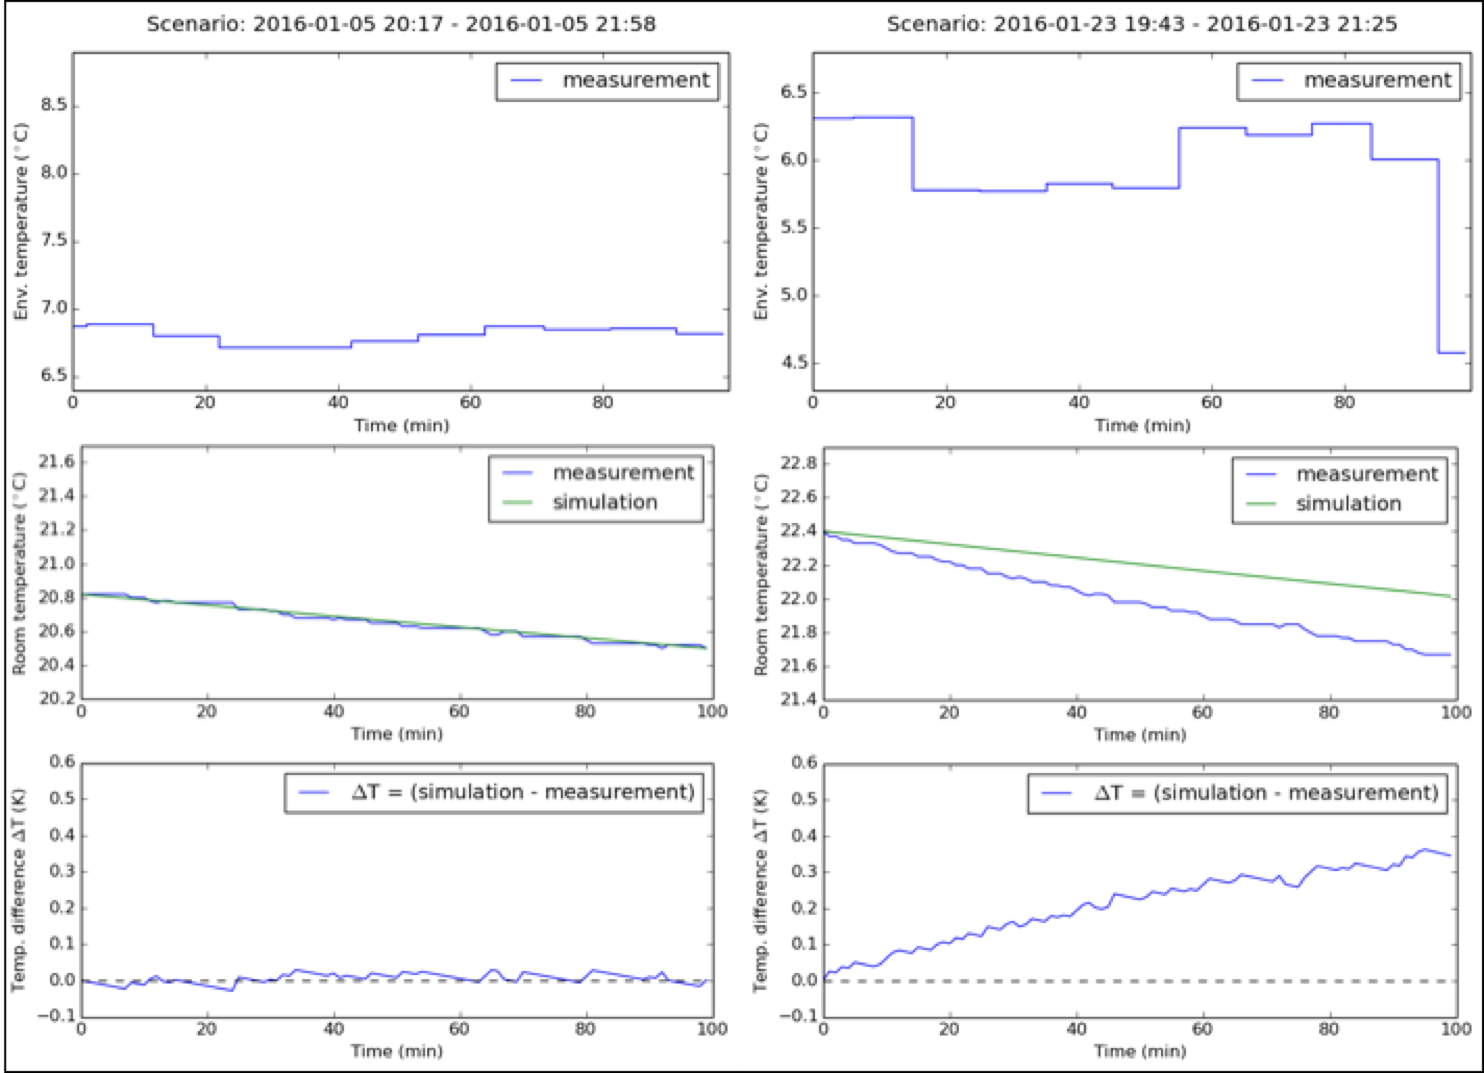
\includegraphics[width=\textwidth]{abbildungen/20160329_pestep1}
\caption{Parameterschätzung des Wärmedurchgangskoeffizienten der Wand in zwei verschiedenen Intervallen}
\label{fig:step1}
\end{figure}

Die Plots auf der linken Seite stellen das Ergebnis für ein 100-minütiges Intervall vom Abend des 05.01.2016, die auf der rechten Seite vom Abend des 23.01.2016 dar. Mit dem vorab fixierten U-Wert für Glas ergab sich ein Schätzwert für den Wärmedurchgangskoeffizient der Wand von $U_{wall}=0.612986$ .

Die oberen beiden Plots zeigen den Verläufe der Steuergröße Außenlufttemperatur, wobei die Solarstrahlung und die Heizung keinen Einfluss hatten. Die genauen Messdaten sind den Dateien auf der angehängten CD in Anhang \ref{att:cd} enthalten. In den mittleren Plots ist ein Vergleich der gemessen Raumtemperatur mit der Simulation des geschätzten Intervalls über 100 Minuten zu finden. Darin ist gut zu erkennen, dass die Dynamik des Modells durch die Anpassung des Parameters verbessert werden konnte. Die unteren Plots zeigen die Abweichung zwischen der Simulation und den Messwerten. Im unteren linken Intervall beschreibt die Simulation, abgesehen von minimalen Abweichungen, das reale System sehr genau. Im rechten Intervall tritt bei der Simulation eine leicht erhöhte Temperatur im Vergleich zur Messung auf, die mit einer Abweichung von etwa $0,35^{\circ}C$ nach 100 Minuten Simulation immer noch eine ausreichende Güte besitzt.

Im nächsten Schritt wird der Transmissionsgrad der Fensterscheiben geschätzt. Dazu wurden Intervalle identifiziert, an denen die Sonne geschienen hat, die Heizung ausgeschaltet war und möglichst wenig Störgrößen aufgetreten sind. Daher bieten sich die Intervalle, am 02.01.2016 und am 05.01.2016 über die Mittagszeit, für eine Schätzung an. In den Zeitintervallen wurde das Büro nur eingeschränkt genutzt wurde, da die Hochschule zu dieser Zeit geschlossen war. Die Ergebnisse der Schätzung sind in \ref{fig:step2} zusammengefasst. Das Skript zur Parameterschätzung findet sich im Anhang \ref{att:cd} in der Datei $room_pe_step2_day.py$.

\begin{figure}
\centering
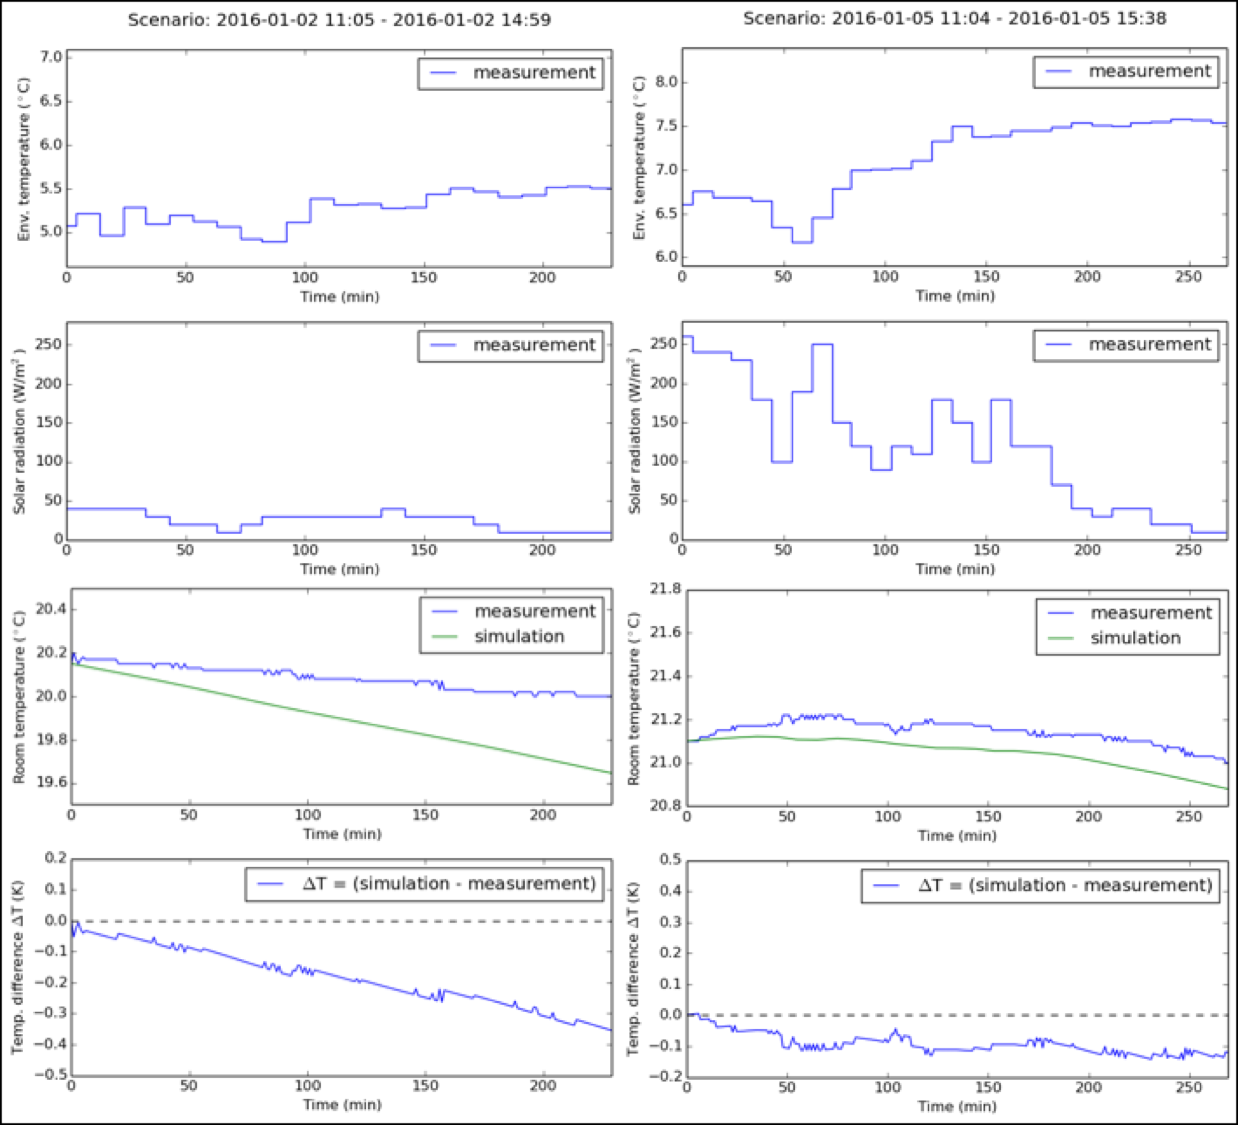
\includegraphics[width=\textwidth]{abbildungen/20160329_pestep2}
\caption{Parameterschätzung}
\label{fig:step2}
\end{figure}

Die Plots auf der linken Seite stellen das Ergebnis für ein 220-minütiges Intervall am 02.01.2016, die auf der rechten Seite für ein 270-minütiges Intervall am 05.01.2016 dar. Die Parameterschätzung ergab einen geschätzten Transmissionsgrad von $window_{transmission}=0.00687213$, der zunächst unrealistisch klein zu sein scheint. Bei einer genaueren Betrachtung ist zu beachten, dass bei der Parameterschätzung eine Anpassung des Modells an die Messwerte stattfindet, also auch deren Störgrößen und Messfehler. Weiterhin ist der tatsächliche Transmissionsgrad der Fensterscheiben in K004b unbekannt, da der Fensterhersteller \textsc{Schüco} lediglich die Rahmen produziert hat. Das Unternehmen, welches die Glasscheiben eingesetzt und die Fenster montiert hat, konnte nicht ermittelt werden. 

In den oberen Plots sind wie in der Abbildung zuvor die Verläufe der Steuergrößen im Schätzintervall zu sehen. Die Außentemperaturen waren in beiden Intervallen mild und lagen zwischen fünf und acht Grad Celsius. im ersten Intervall wurde eine schwache, im zweiten hingegen eine starke Globalstrahlung gemessen. Auf beiden Ergebnisplots ist zu erkennen, dass der Einfluss der Strahlung zum Ende des Intervalls hin immer weiter unterschätzt wird. Die Temperaturabweichung liegt in beiden Intervallen kleiner $0,4^{\circ}C$. Im rechten Modellabgleich lässt sich durch die leicht angedeuteten Senken erkennen, dass das Verhalten des Modells mit der Realität trotz Abweichungen sehr gut abgebildet wird.
Da insbesondere die ersten Minuten der Simulation eine ausreichende Beschreibung der Realität liefern und die Temperaturkurve mit Messfehlern behaftet ist, reicht die Güte des Modells für eine Anwendung einer Modellprädiktiven Regelung aus. 


Um eine Einordnung der verbesserten Modellgüte zu erhalten, erfolgt eine erneute Simulation des ersten Validierungsintervalls ohne den Einsatz eines Heizkörper. Die Ergebnisse sind im Plot in \ref{fig:valid1pe} dargestellt.

\begin{figure}
\centering
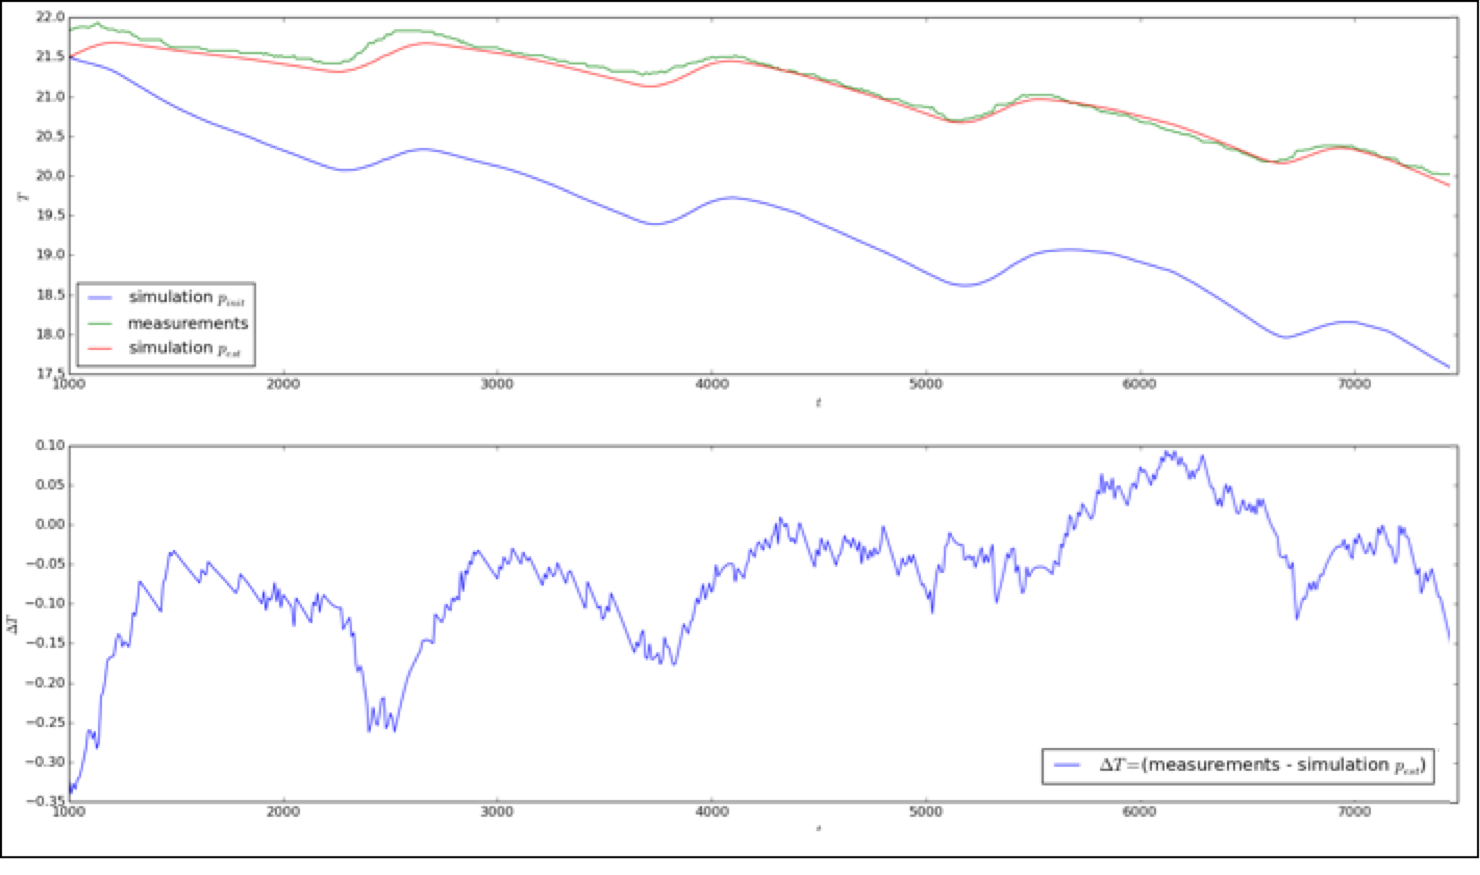
\includegraphics[width=\textwidth]{abbildungen/20160329_validierung1pe}
\caption{Simulation des Raummodells ohne Einsatz der Heizung mit geschätzten Parametern}
\label{fig:valid1pe}
\end{figure}

Abgesehen von einem Fehler bei der Initialisierung der Raumtemperatur zu Beginn der Simulation, ist eine erheblich Verbesserung der Modellgüte zu erkennen. Die Abweichung der Simulation ist über das gesamte fünftägige Intervall sehr gering und die Dynamik des Systems wird sehr genau beschrieben.

Im letzten Schritt wird die Schätzung des Wärmedurchgangskoeffizienten des Heizkörpers durchgeführt. Es wurden erneut geeignete Schätzintervalle identifiziert, an denen keine Solarstrahlung zu finden war und möglichst keine Störgrößen auftraten. Dazu boten sich speziell zwei Intervalle am Abend des 17.01.2016 an, an dem die Heizung von der Anlage genutzt wurde. Die Ergebnisse der Parameterschätzung für die beiden 20 Minuten umfassenden Intervalle sind in \ref{fig:step3} abgebildet. Das Skript zur Parameterschätzung findet sich im Anhang \ref{att:cd} in der Datei $room_pe_step3_radiator_night.py$.

\begin{figure}
\centering
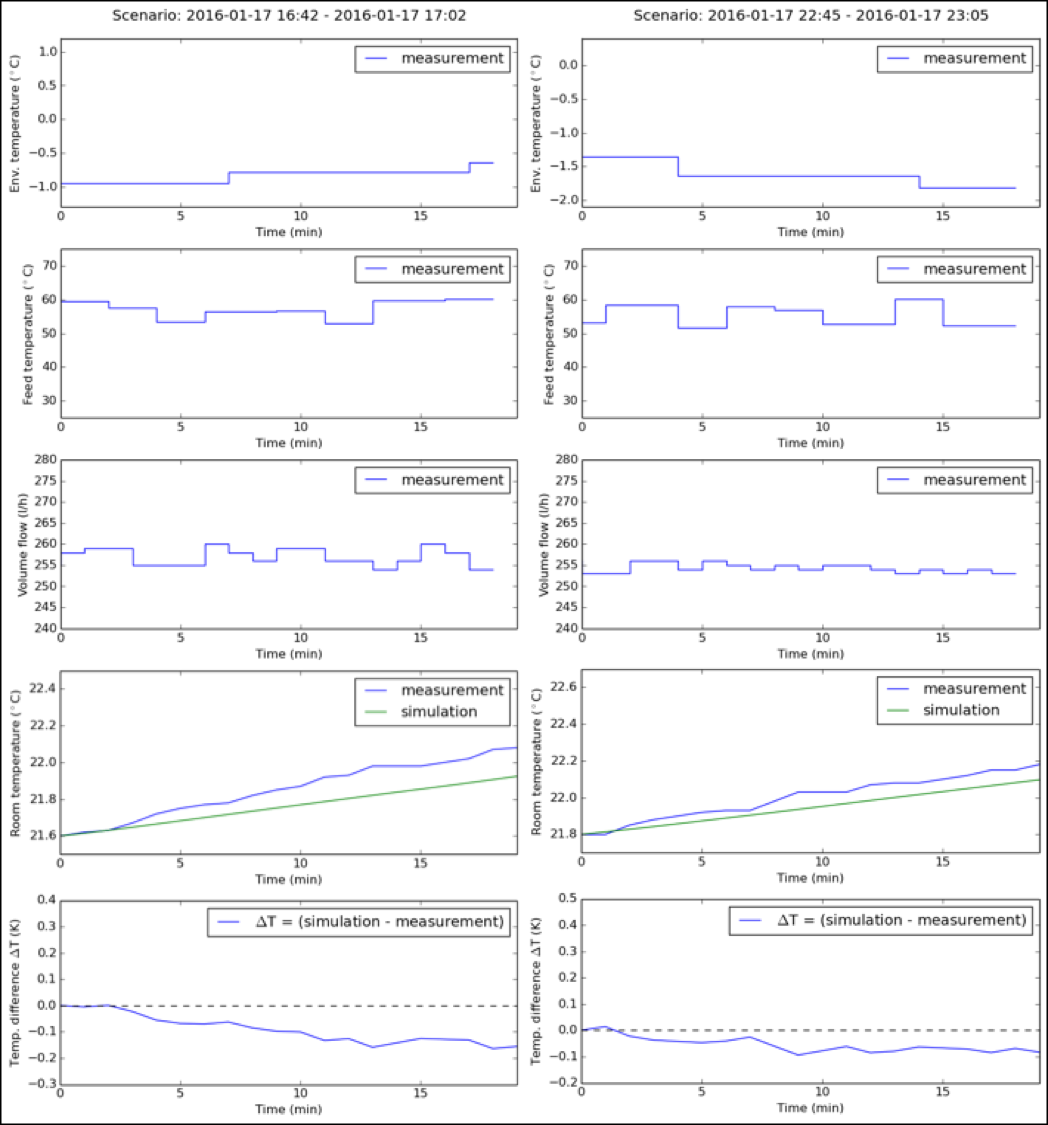
\includegraphics[width=\textwidth]{abbildungen/20160329_pestep3}
\caption{Parameterschätzung}
\label{fig:step3}
\end{figure}

Die Plots stellen das Ergebnis für die beiden 20-minütigen Intervalle dar. Die Parameterschätzung ergab einen realistischen Schätzwert für den Wärmedurchgangskoeffizienten des Heizkörpers von $u=_{radiator}=12.9872$.
Wie zuvor sind in den oberen Plots die Verläufe der Steuergrößen im Schätzintervall zu sehen. Die Außentemperaturen waren in beiden Intervallen knapp unterhalb des Gefrierpunkts. In keinem der beiden Intervalle wurde eine Globalstrahlung gemessen. Außerdem wurde die Heizung mit voller Leistung betrieben.
Auf beiden Ergebnisplots folgt die Simulation der Temperaturkurve ziemlich exakt, wenn auch die Diskrepanz zum Ende des Intervalls hin zunimmt. Mit einer maximalen Temperaturabweichung von $0,2^{\circ}C$ in beiden Intervallen, beschreibt das Modell das reale Verhalten damit ausreichend.

Eine erneute Simulation des vorherigen Simulationsintervalls mit dem Einsatz des Heizkörper, das in \ref{fig:valid2} dargestellt ist, verdeutlicht eine Verbesserung des Modells. Die Ergebnisse werden im Plot in \ref{fig:valid2pe} aufgezeigt.

\begin{figure}
\centering
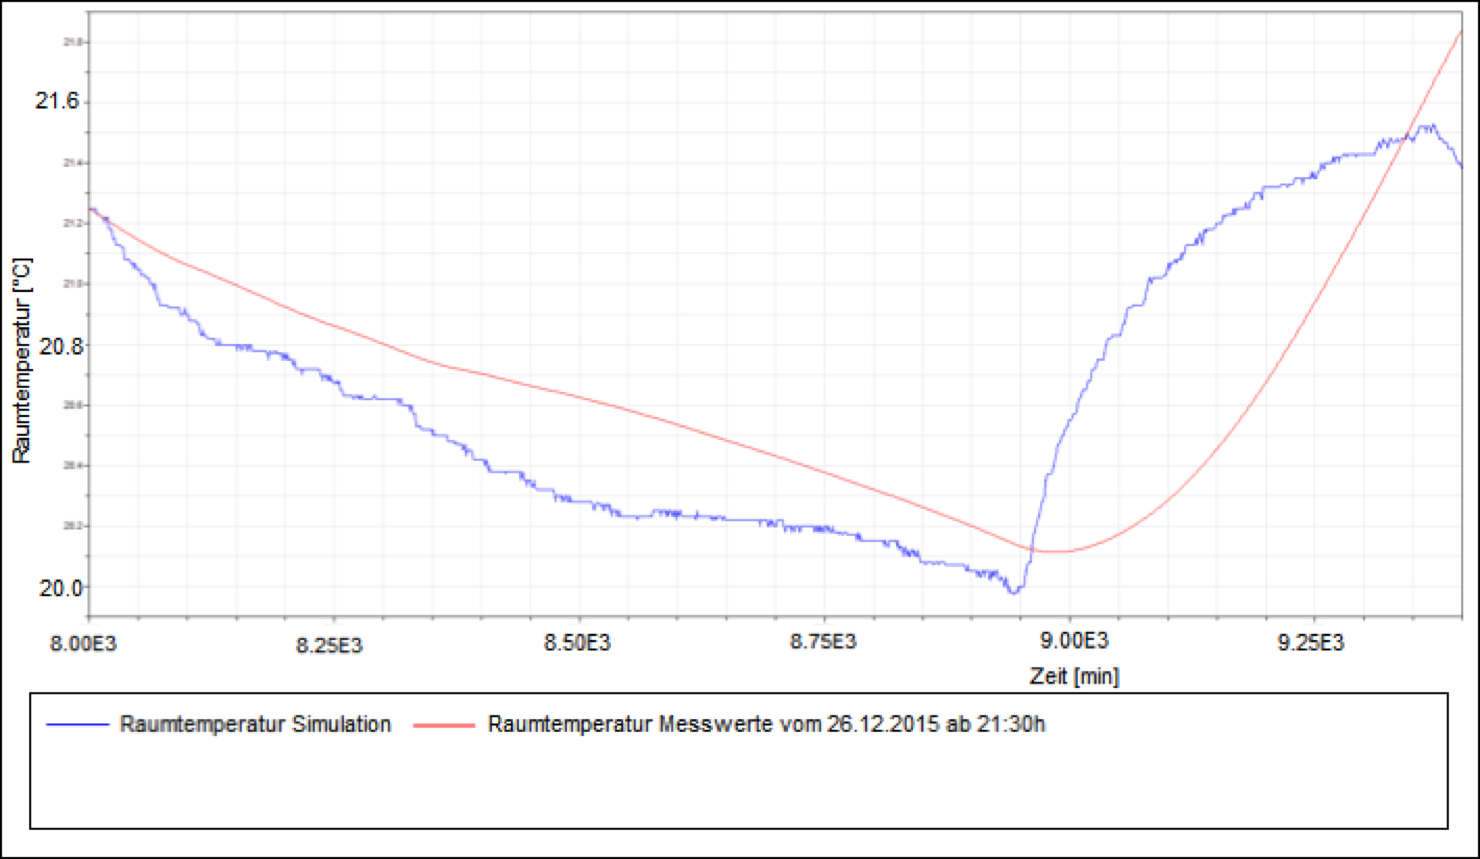
\includegraphics[width=\textwidth]{abbildungen/20160330_validierung2pe}
\caption{Simulation des Raummodells mit Einsatz des Heizkörpers mit geschätzten Parametern}
\label{fig:valid2pe}
\end{figure}

Die Abweichungen der Kurve sind deutlich verbessert und auch die zeitliche Verzögerung hat sich verkürzt. Die Dynamik hat sich für das eintägige Intervall ebenfalls verbessert, wenn auch nur leicht. 

Abschließend erfolgt eine Modellprädiktive regelungsnahe Simulation des Modells. Das Ergebnis ist in \ref{fig:bench} dargestellt.

\begin{figure}
\centering
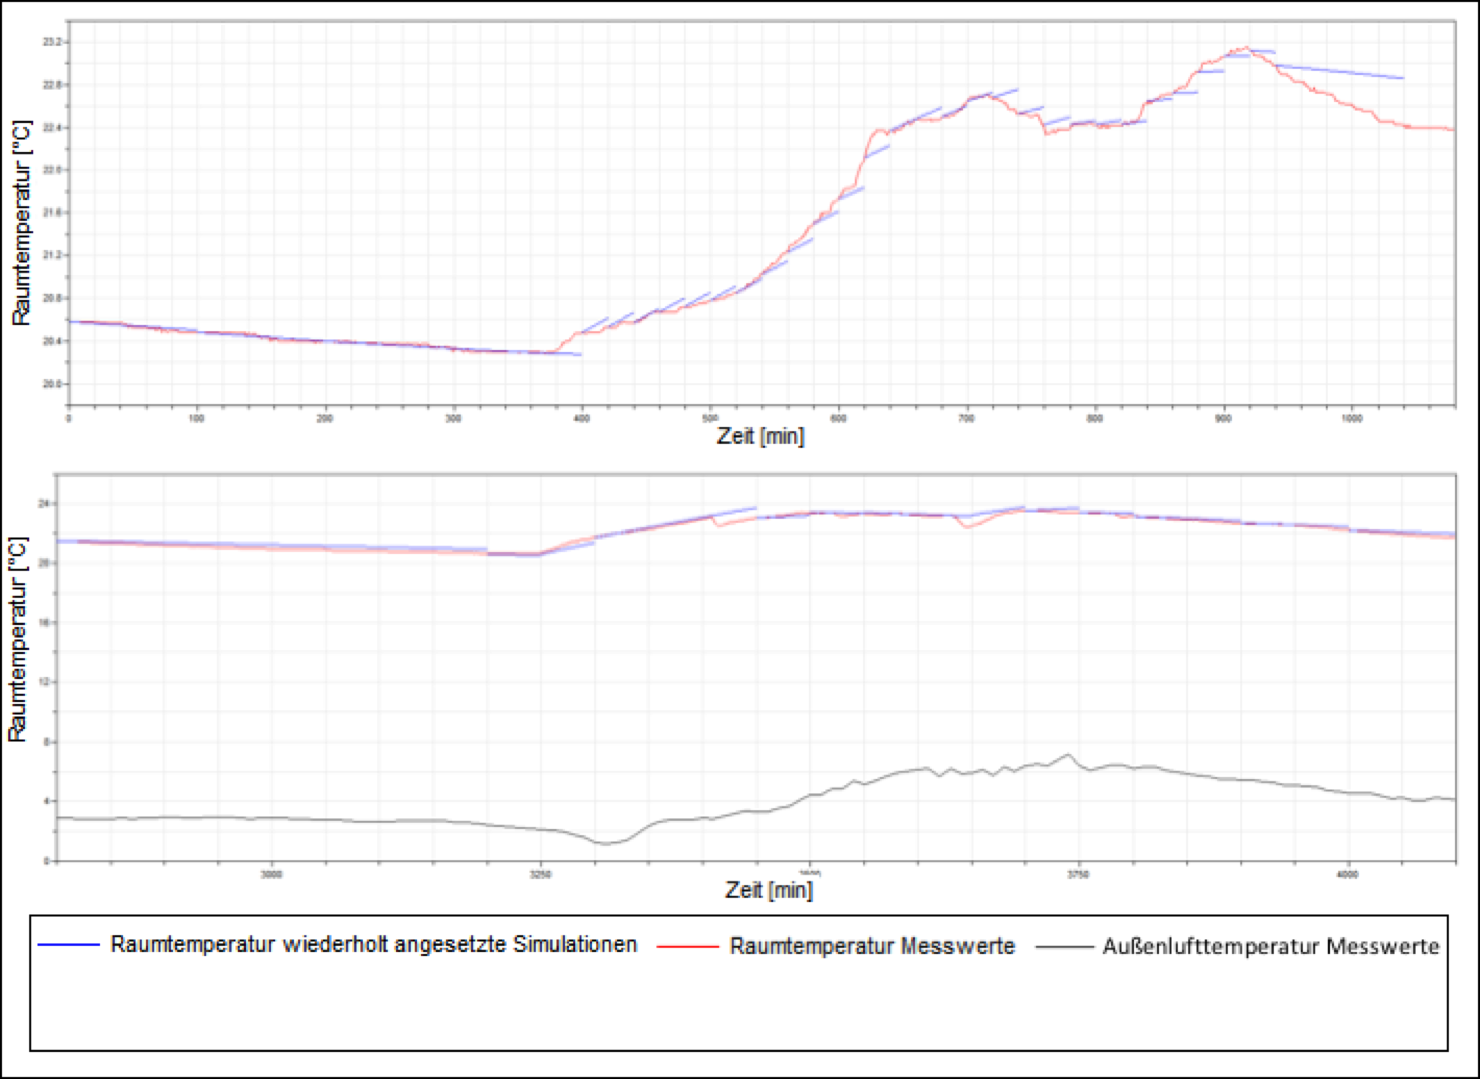
\includegraphics[width=\textwidth]{abbildungen/20160330_benchmark}
\caption{Simulation des Raummodells mit Einsatz des Heizkörpers mit geschätzten Parametern}
\label{fig:bench}
\end{figure}

Es wurden wiederholt kürzere Simulationen mit einer angepassten Initialtemperatur angesetzt, um eine der Modellprädiktiven Regelung ähnelnde Simulation zu erhalten. Die Außenlufttemperatur bewegte sich während des Zeitraums knapp über dem Gefrierpunkt und es wurde lediglich eine schwache Globalstrahlung detektiert. Beim Einsatz der Heizung wurden kürzere Simulationsintervalle von 20 Minuten angenommen, für die restlichen Simulationen wurden hingegen längere Intervalle angesetzt.
Nach 800 simulierten Minuten setzt die Heizung ein, was durch das Modell gut abgebildet wird. Es bestehen lediglich Abweichungen bei zwei kleineren Temperaturabfällen, die sich durch Störgrößen wie beispielsweise das Öffnen der Fenster erklären lassen, und daher vom Modell nicht berücksichtigt wurden.

Zusammenfassend lässt sich festhalten, dass das Modell eine solide Beschreibung des Verhaltens von K004b liefert und sich damit für den Einsatz mit einer \acrlong{mpr} eignet. Im letzten Abschnitt wird überprüft, ob das Modell den Anforderungen für den Einsatz mit \textsc{JModelica.org} genügt.

\section{Modellprädiktive Regelung}

Um eine \acrlong{mpr} in \textsc{\textsc{JModelica.org}} anhand des Raummodells zu ermöglichen, wird das Modell in ein optimierungsfähiges Objekt übersetzt. Dazu wird das Modell mithilfe des \textsc{JModelica.org} Compilers anhand des Programms in Listing \ref{lst:comp} in ein JMU und Optimization Object transferiert.

\lstinputlisting[language=Python ,caption={Programm zur Übersetzung des Raummodells in optimierungsfähige Objekte in \textsc{JModelica.org}}, label=lst:comp]{listings/compiling.py}

Trotz der Ausgabe von kleineren Warnungen, lässt sich das Modell fehlerfrei übersetzen und damit für Optimierungszwecke in \textsc{JModelica.org} nutzen. Eine Bestätigung des erfolgreich übersetzten Problems findet sich in der Python Konsole in \ref{fig:jmod}.

\begin{figure}
\centering
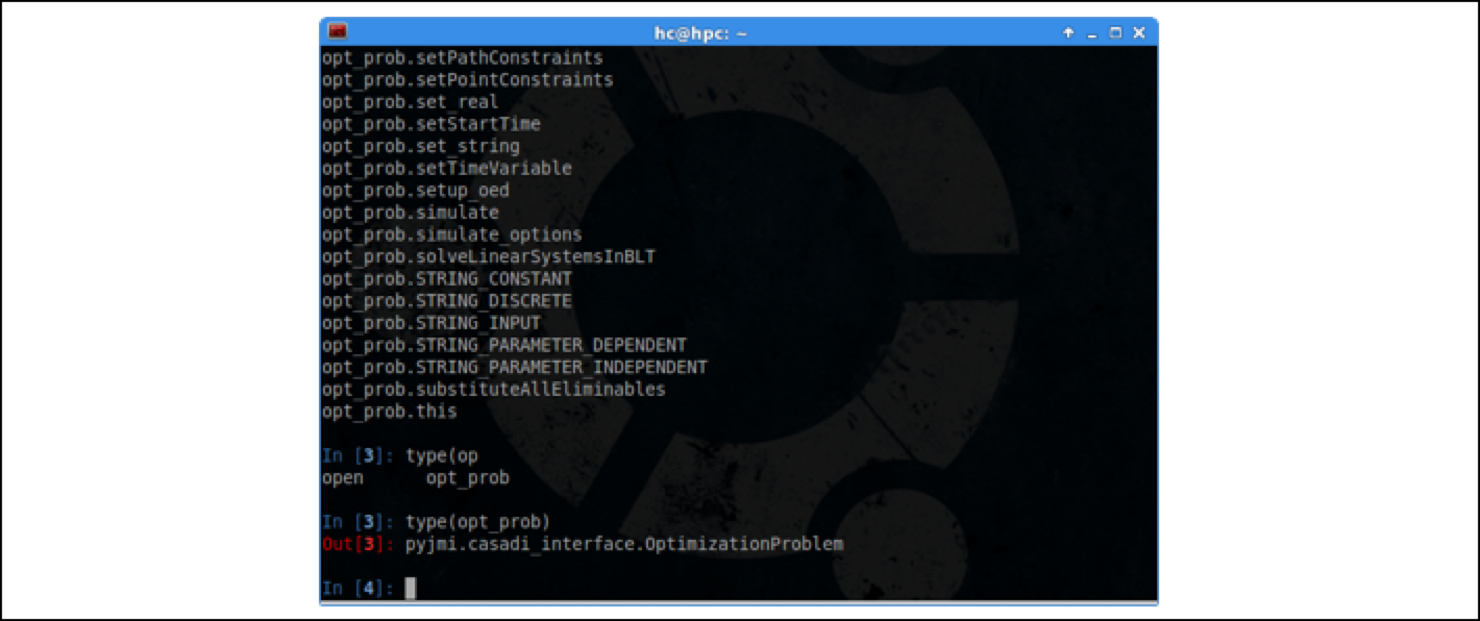
\includegraphics[width=\textwidth]{abbildungen/20160330_mpc}
\caption{\textsc{\textsc{JModelica.org}} Kompatibilität des Modells}
\label{fig:jmod}
\end{figure}

Die Hypothese, dass sich das Modell für den Einsatz mit \textsc{JModelica.org} eignet, kann also bestätigt werden.
Damit sind die Voraussetzungen für eine Modellprädiktive Regelung der Raumtemperatur in K004b geschaffen.